%%%%%%%%%%%%%%%%%%%%%%%%%%%%%%%%%%%%%%%%%%%%%%%%%%%%%%%%%%%%%%%%%%%%%%%%
%                                                                      %
%     File: Thesis_Appendix_A.tex                                      %
%     Tex Master: Thesis.tex                                           %
%                                                                      %
%     Author: Andre C. Marta                                           %
%     Last modified : 27 Feb 2024                                      %
%                                                                      %
%%%%%%%%%%%%%%%%%%%%%%%%%%%%%%%%%%%%%%%%%%%%%%%%%%%%%%%%%%%%%%%%%%%%%%%%

\chapter{Best-so-far correction}
\label{Appendix:BestSoFarCorrection}

Here are the revised plots illustrating the median best-so-far metric for the numerous heuristics tested throughout this study.

% Swap these things' order. Put the 4 plots for the 32 and 100-node graphs in the first page, and the remaining 5 go on the other page. This way, I shouldn't have to worry about these mismatches in size.

% Fix this tomorrow: sizes and labeling of the subfigures (a), (b), etc. are off. Fix this tomorrow (20/05).

\begin{figure*}[hb!]
    \centering
    \begin{subfigure}[t]{0.495\textwidth}
		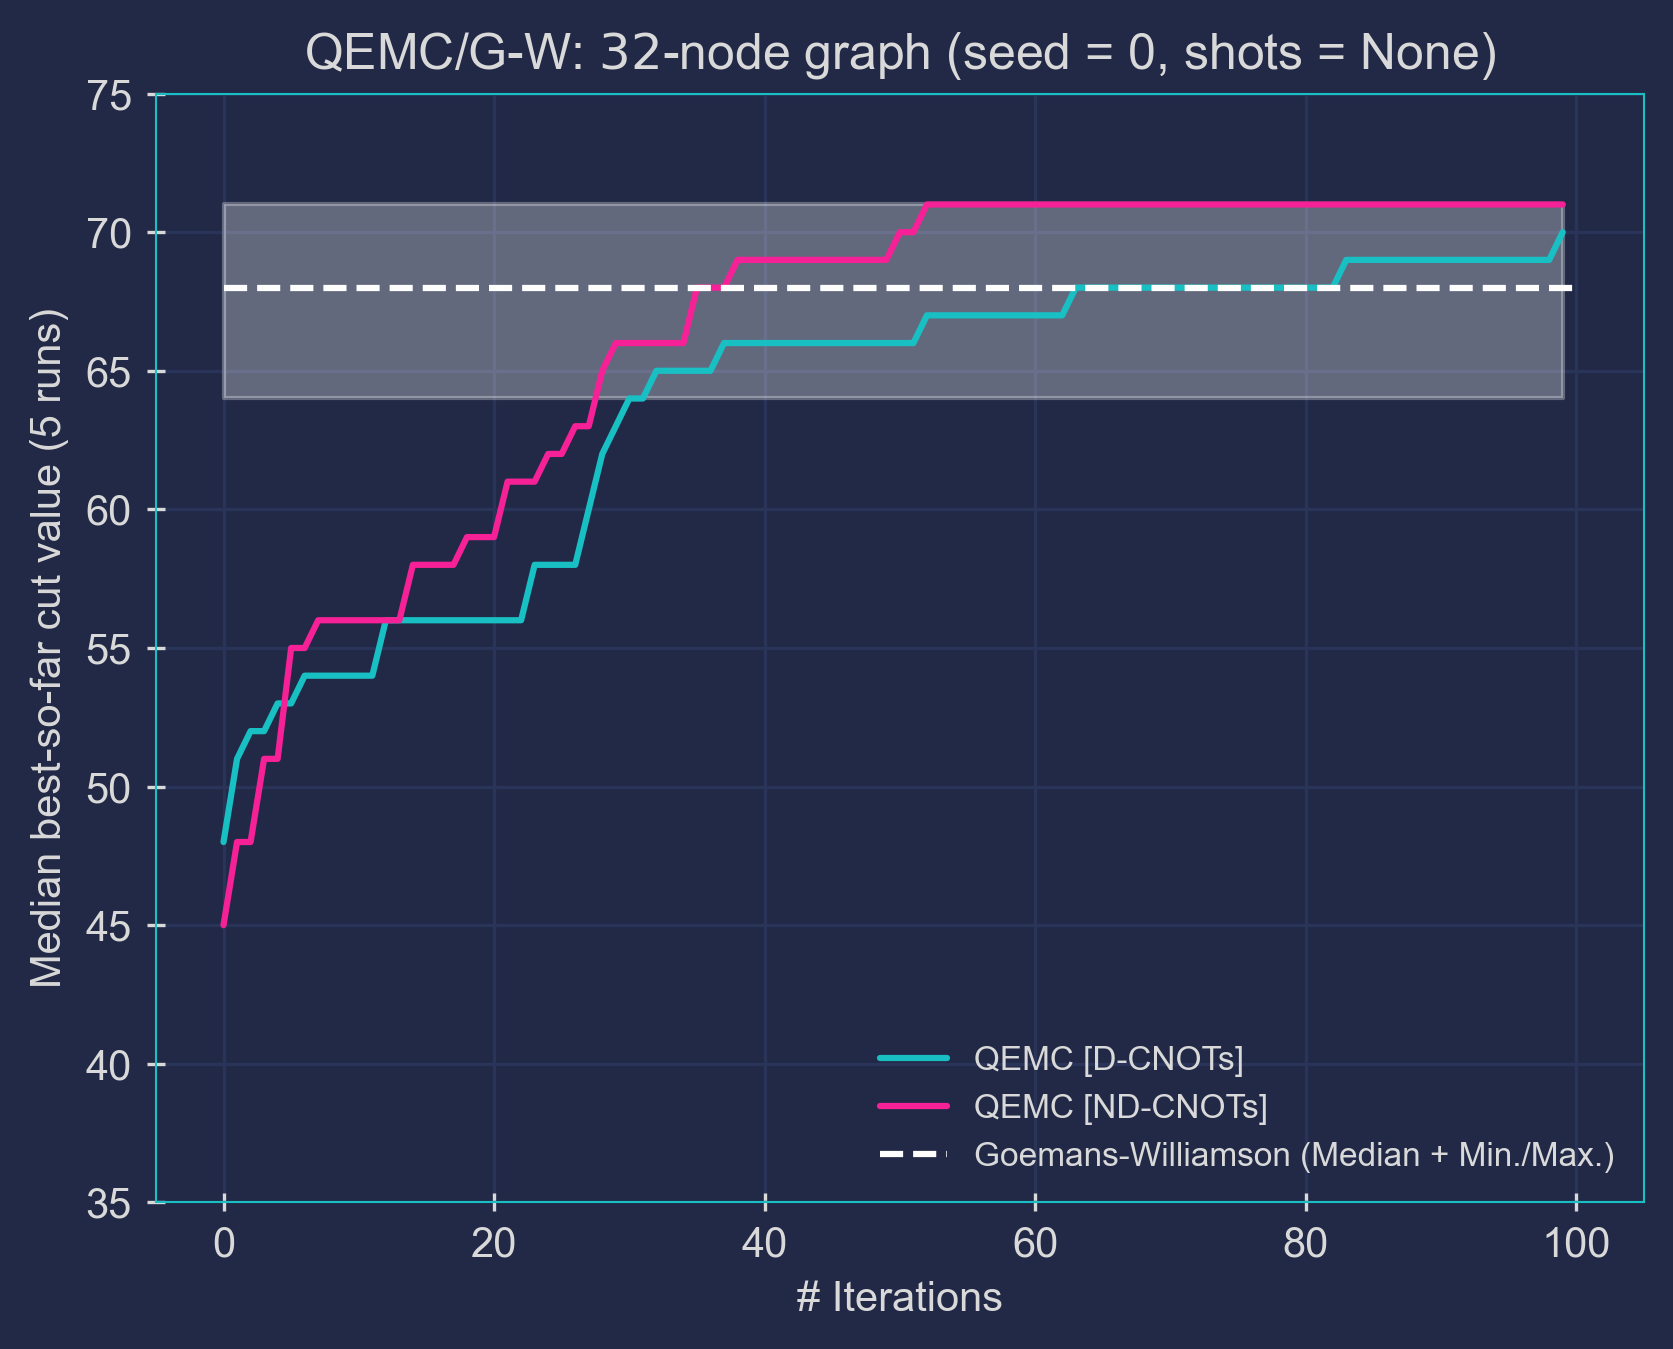
\includegraphics[width=0.975\textwidth, height=0.75\textwidth]{Figures/Appendix_A/32-node/32-node_Graph(QEMC&G-W)_Updated.png}
		\caption{$32$-node graph – \acrshort{qemc} and \acrshort{gw} exclusively.}
		\label{fig:C_BSF_1_32-node}
	\end{subfigure}
    \hfill
    \begin{subfigure}[t]{0.495\textwidth}
		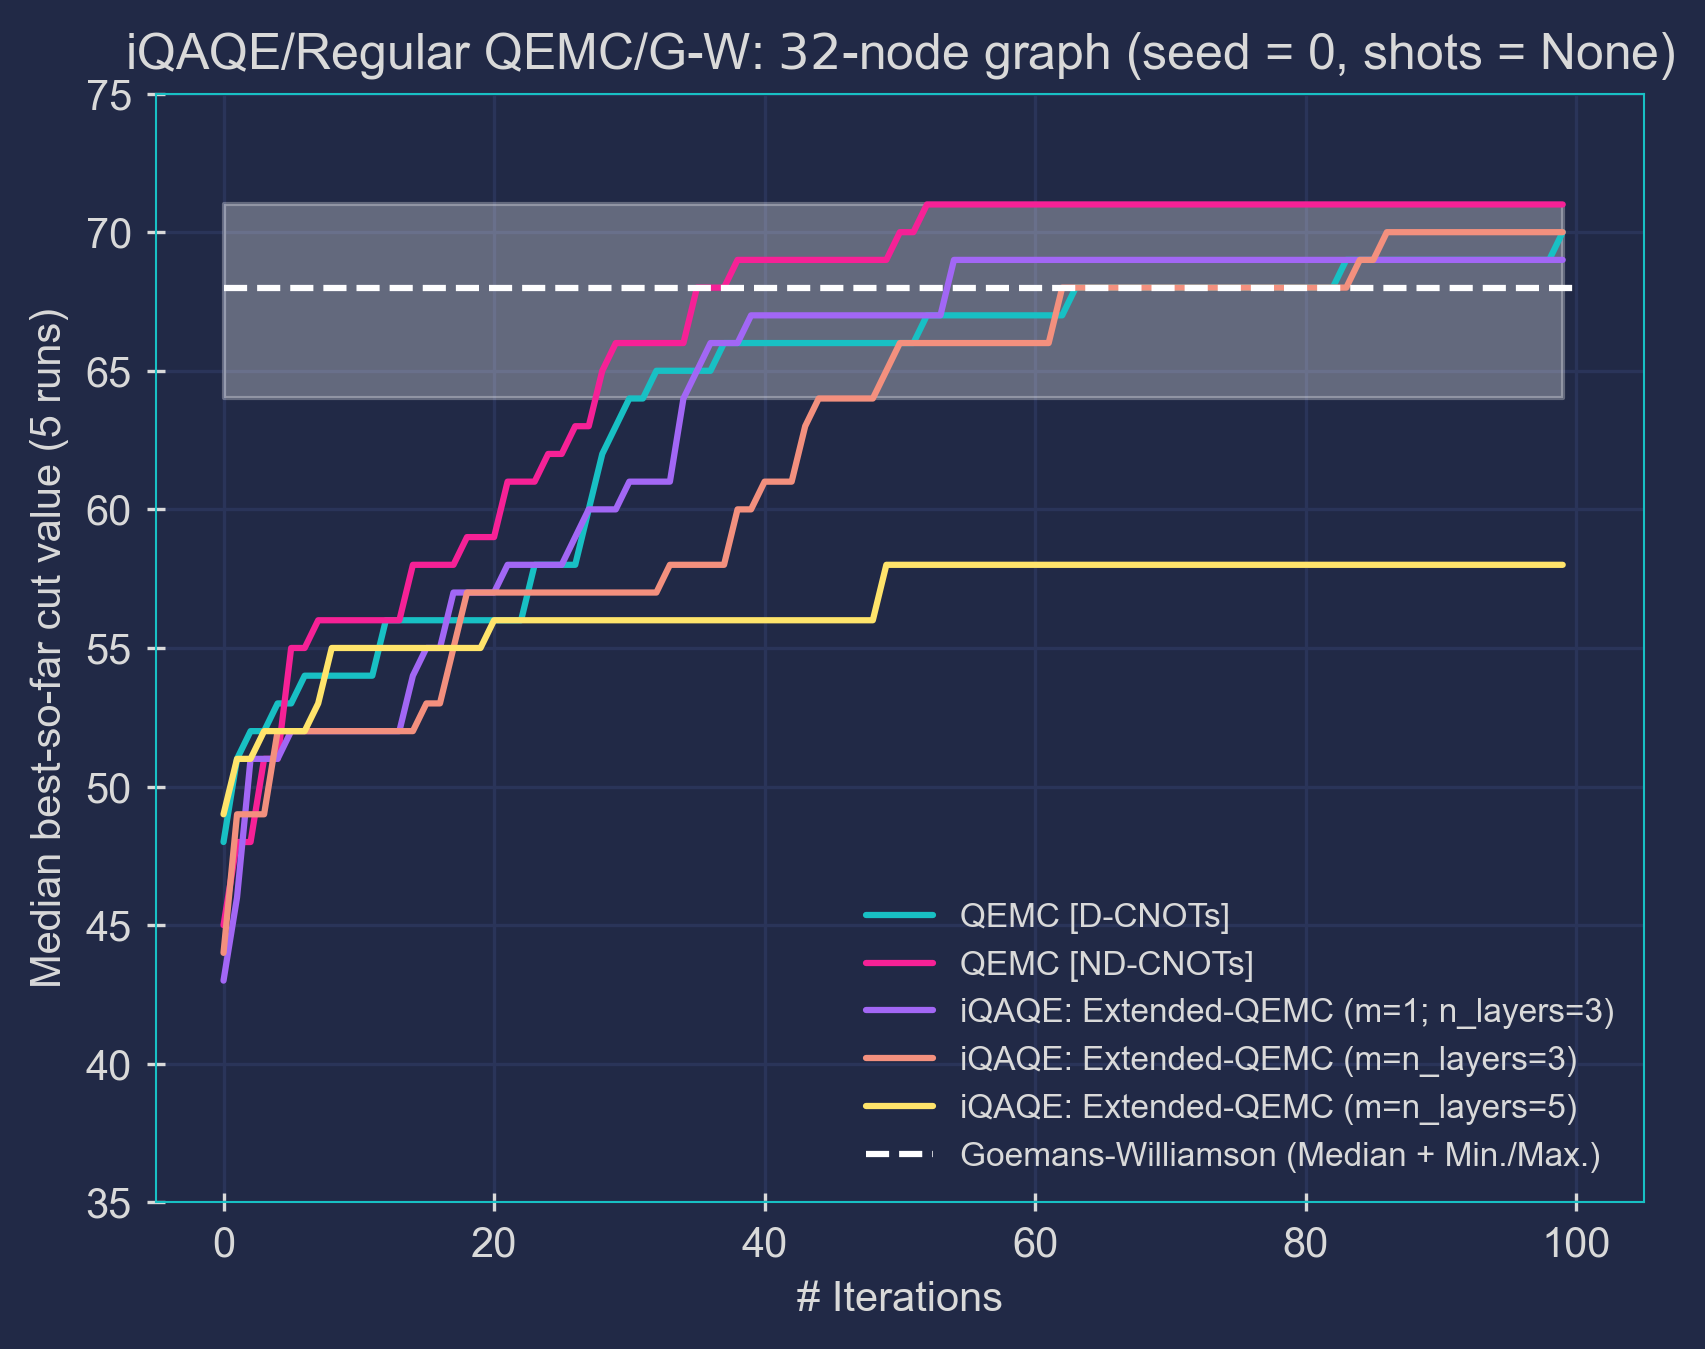
\includegraphics[width=0.975\textwidth, height=0.75\textwidth]{Figures/Appendix_A/32-node/32-node_Graph_Updated.png}
		\caption{$32$-node graph – other schemes.}
		\label{fig:C_BSF_2_32-node}
	\end{subfigure}

    \bigskip

    \begin{subfigure}[t]{0.495\textwidth}
		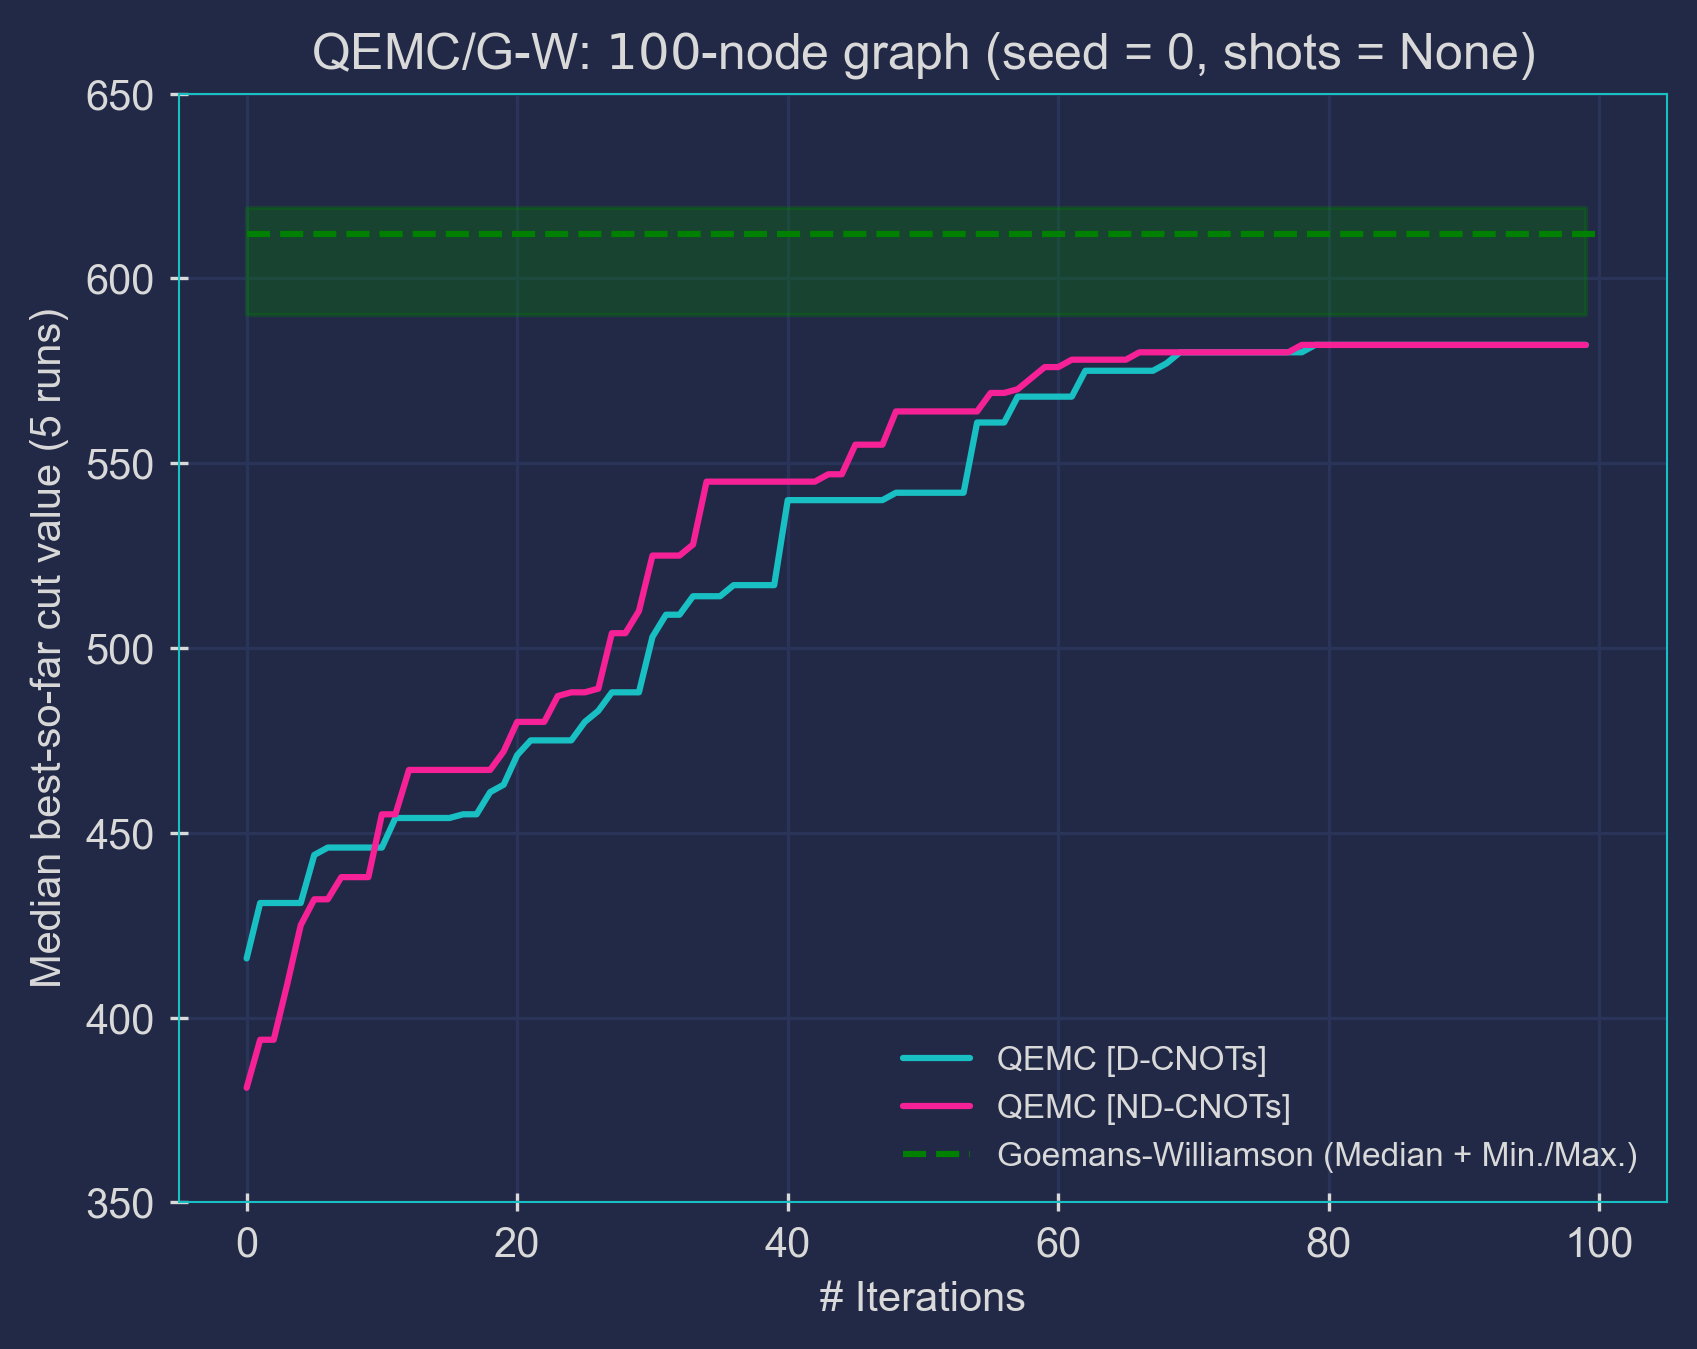
\includegraphics[width=0.975\textwidth, height=0.75\textwidth]{Figures/Appendix_A/100-node/100-node_Graph(QEMC&G-W)_Updated.png}
		\caption{$100$-node graph – \acrshort{qemc} and \acrshort{gw} exclusively.}
		\label{fig:C_BSF_1_100-node}
	\end{subfigure}
    \hfill
    \begin{subfigure}[t]{0.495\textwidth}
		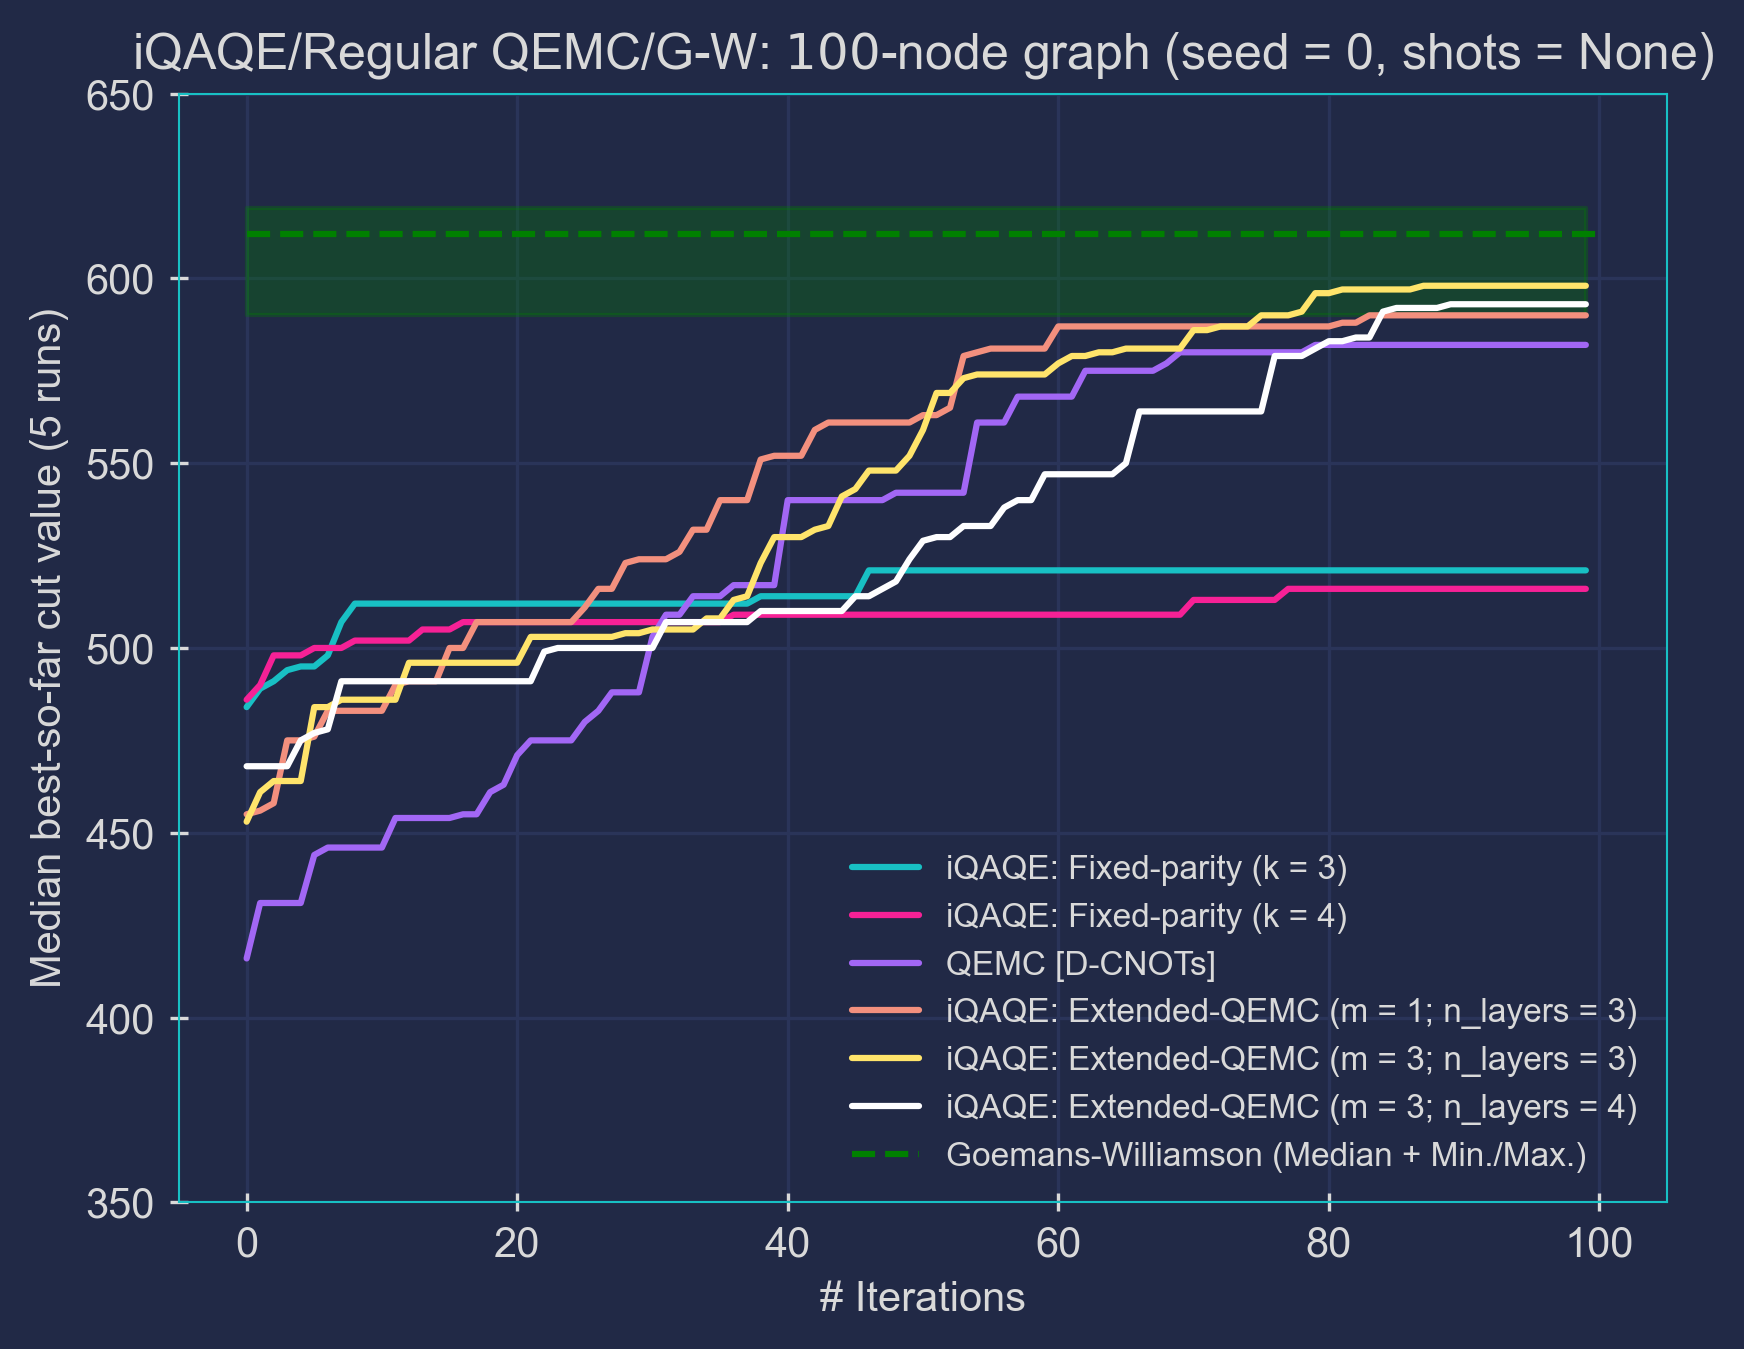
\includegraphics[width=0.975\textwidth, height=0.75\textwidth]{Figures/Appendix_A/100-node/100-node_Graph_Updated.png}
		\caption{$32$-node graph – other schemes.}
		\label{fig:C_BSF_2_100-node}
	\end{subfigure}
    \caption{Revised results using the median best-so-far metric for the $32$ and $100$-node graphs.}
    \label{fig:Corrected_BSF_Results_8-node}
\end{figure*}

\clearpage

\begin{figure*}
    \begin{subfigure}[t]{0.495\textwidth}
        \centering
        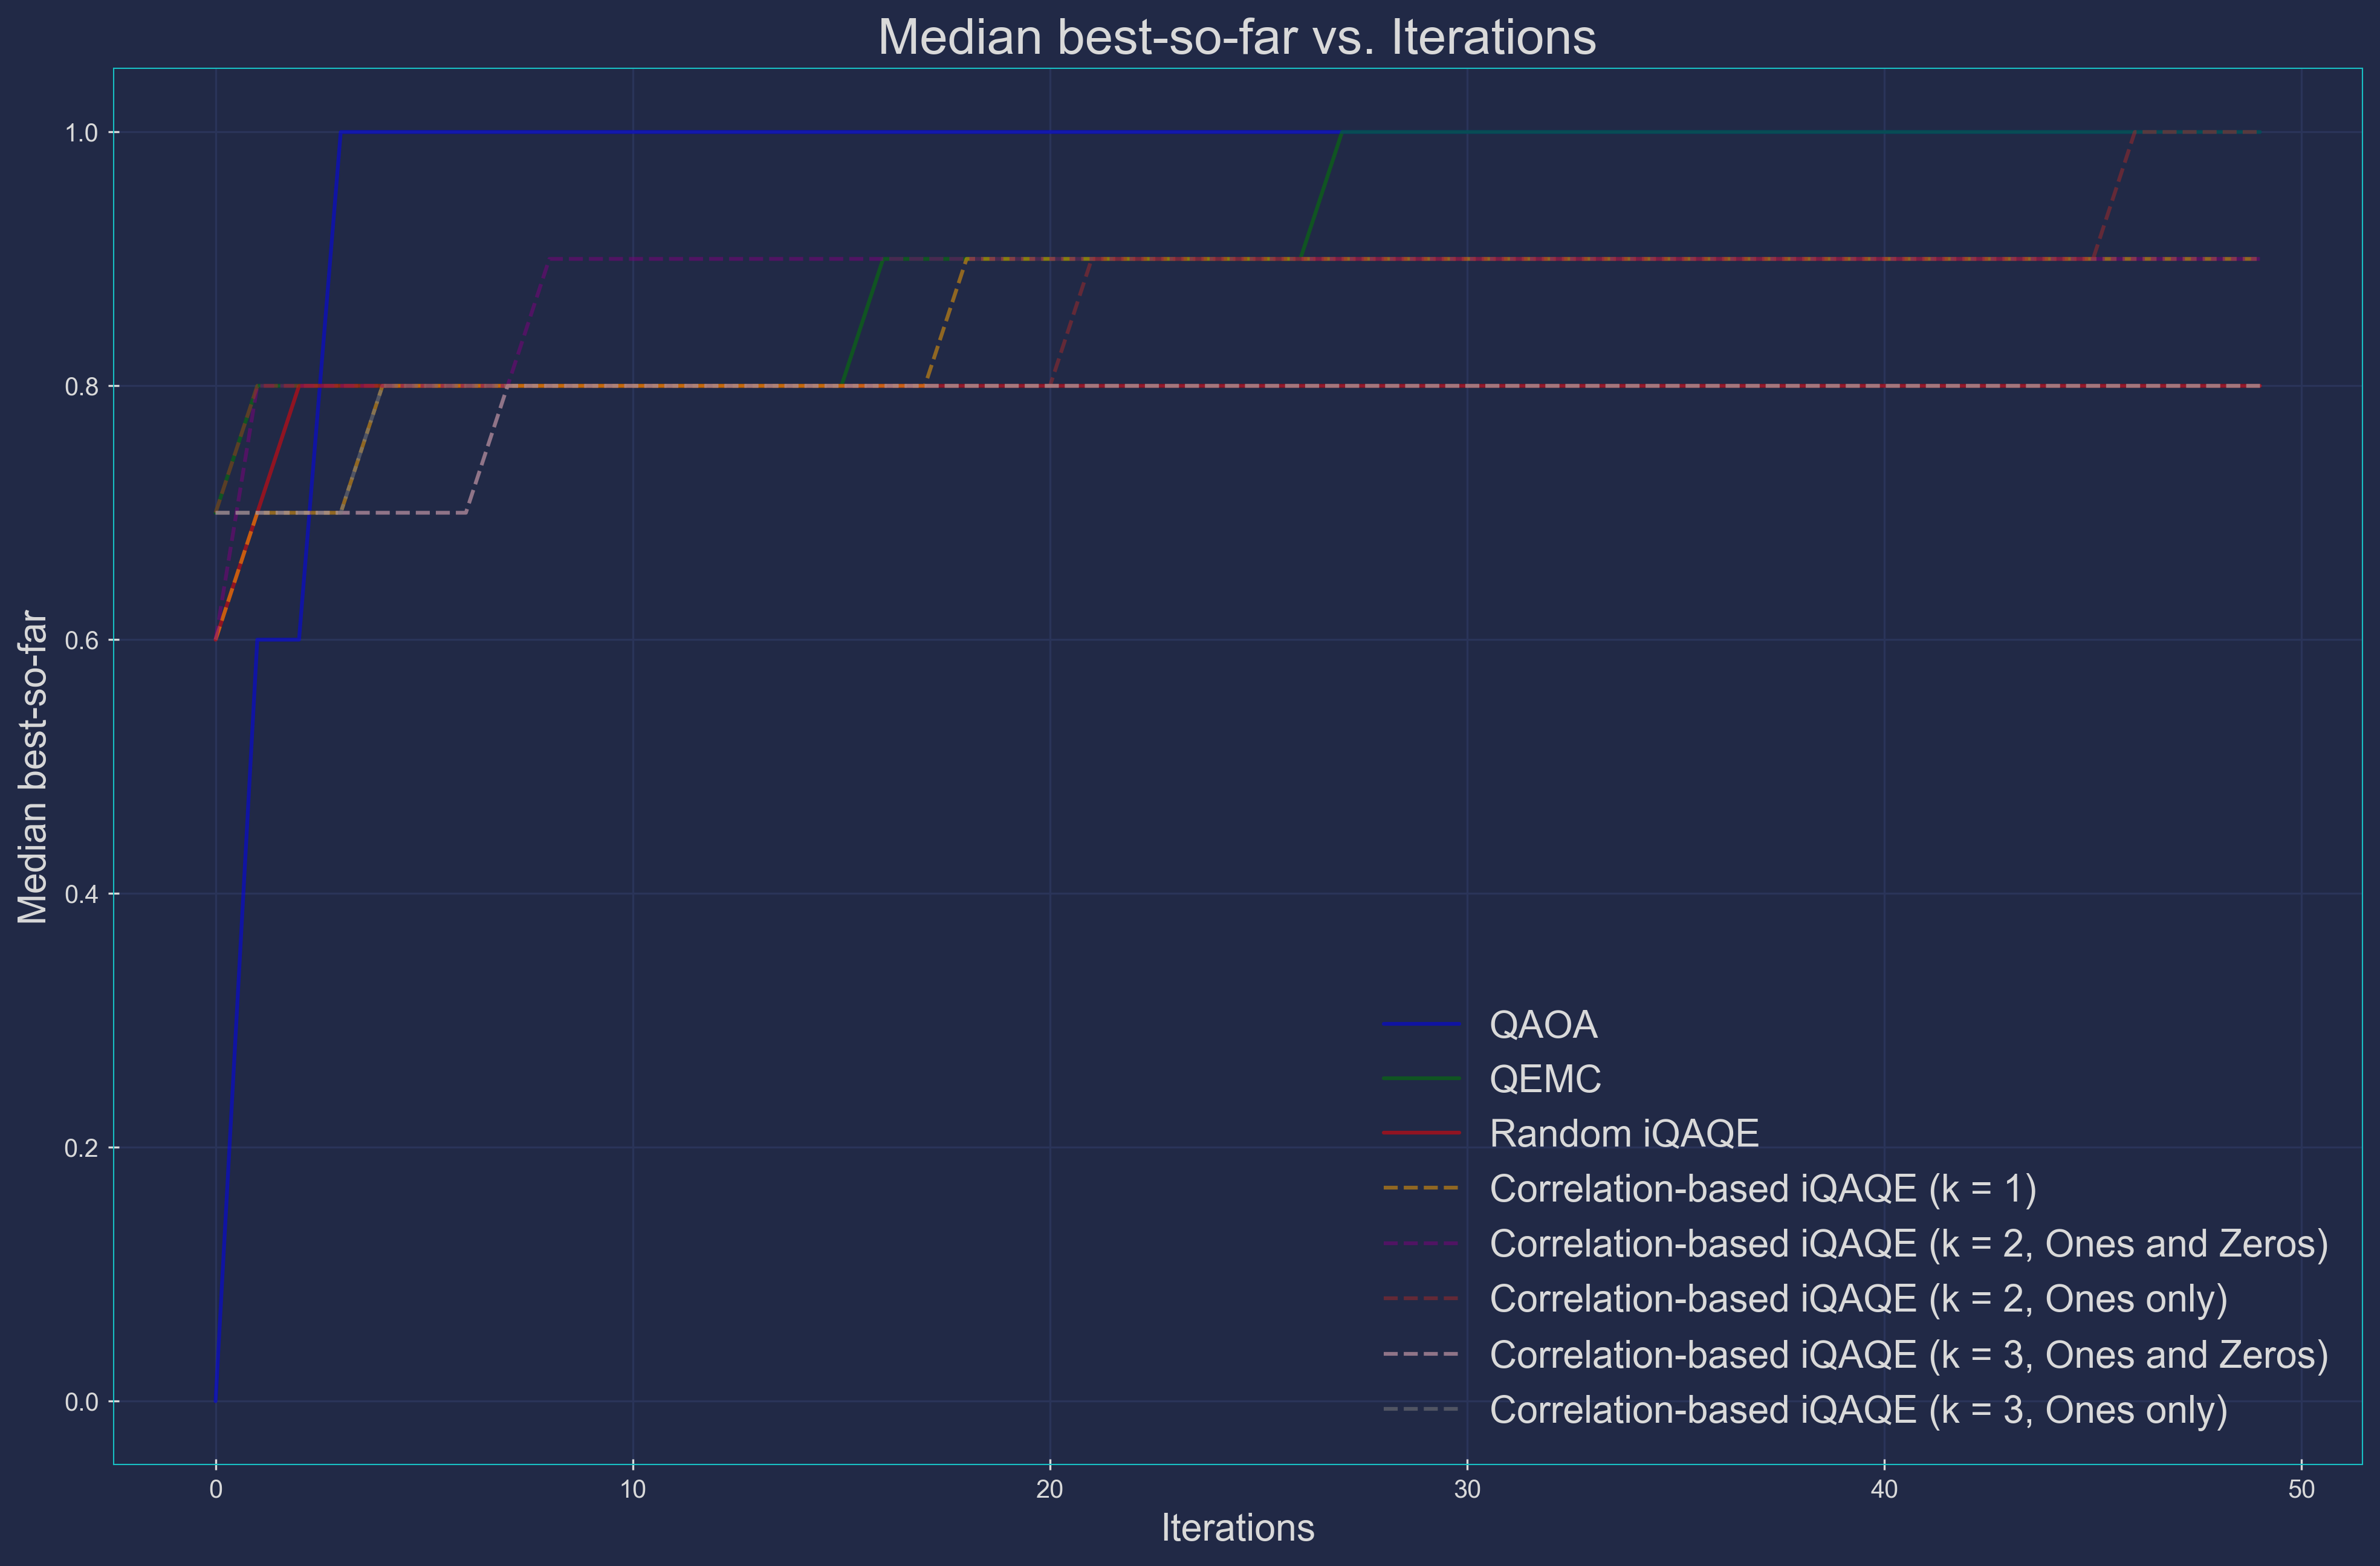
\includegraphics[width=0.975\textwidth]{Figures/Appendix_A/8-node/Basic+Correlation_iQAQE(8-node).png}
        \caption{\raggedright Correlation-based schemes compared to \acrshort{qaoa}, \acrshort{qemc}, and a randomly chosen \acrshort{iqaqe} instance.}
        \label{fig:C_BSF_1_8-node}
    \end{subfigure}
    \hfill
    \begin{subfigure}[t]{0.495\textwidth}
        \centering
        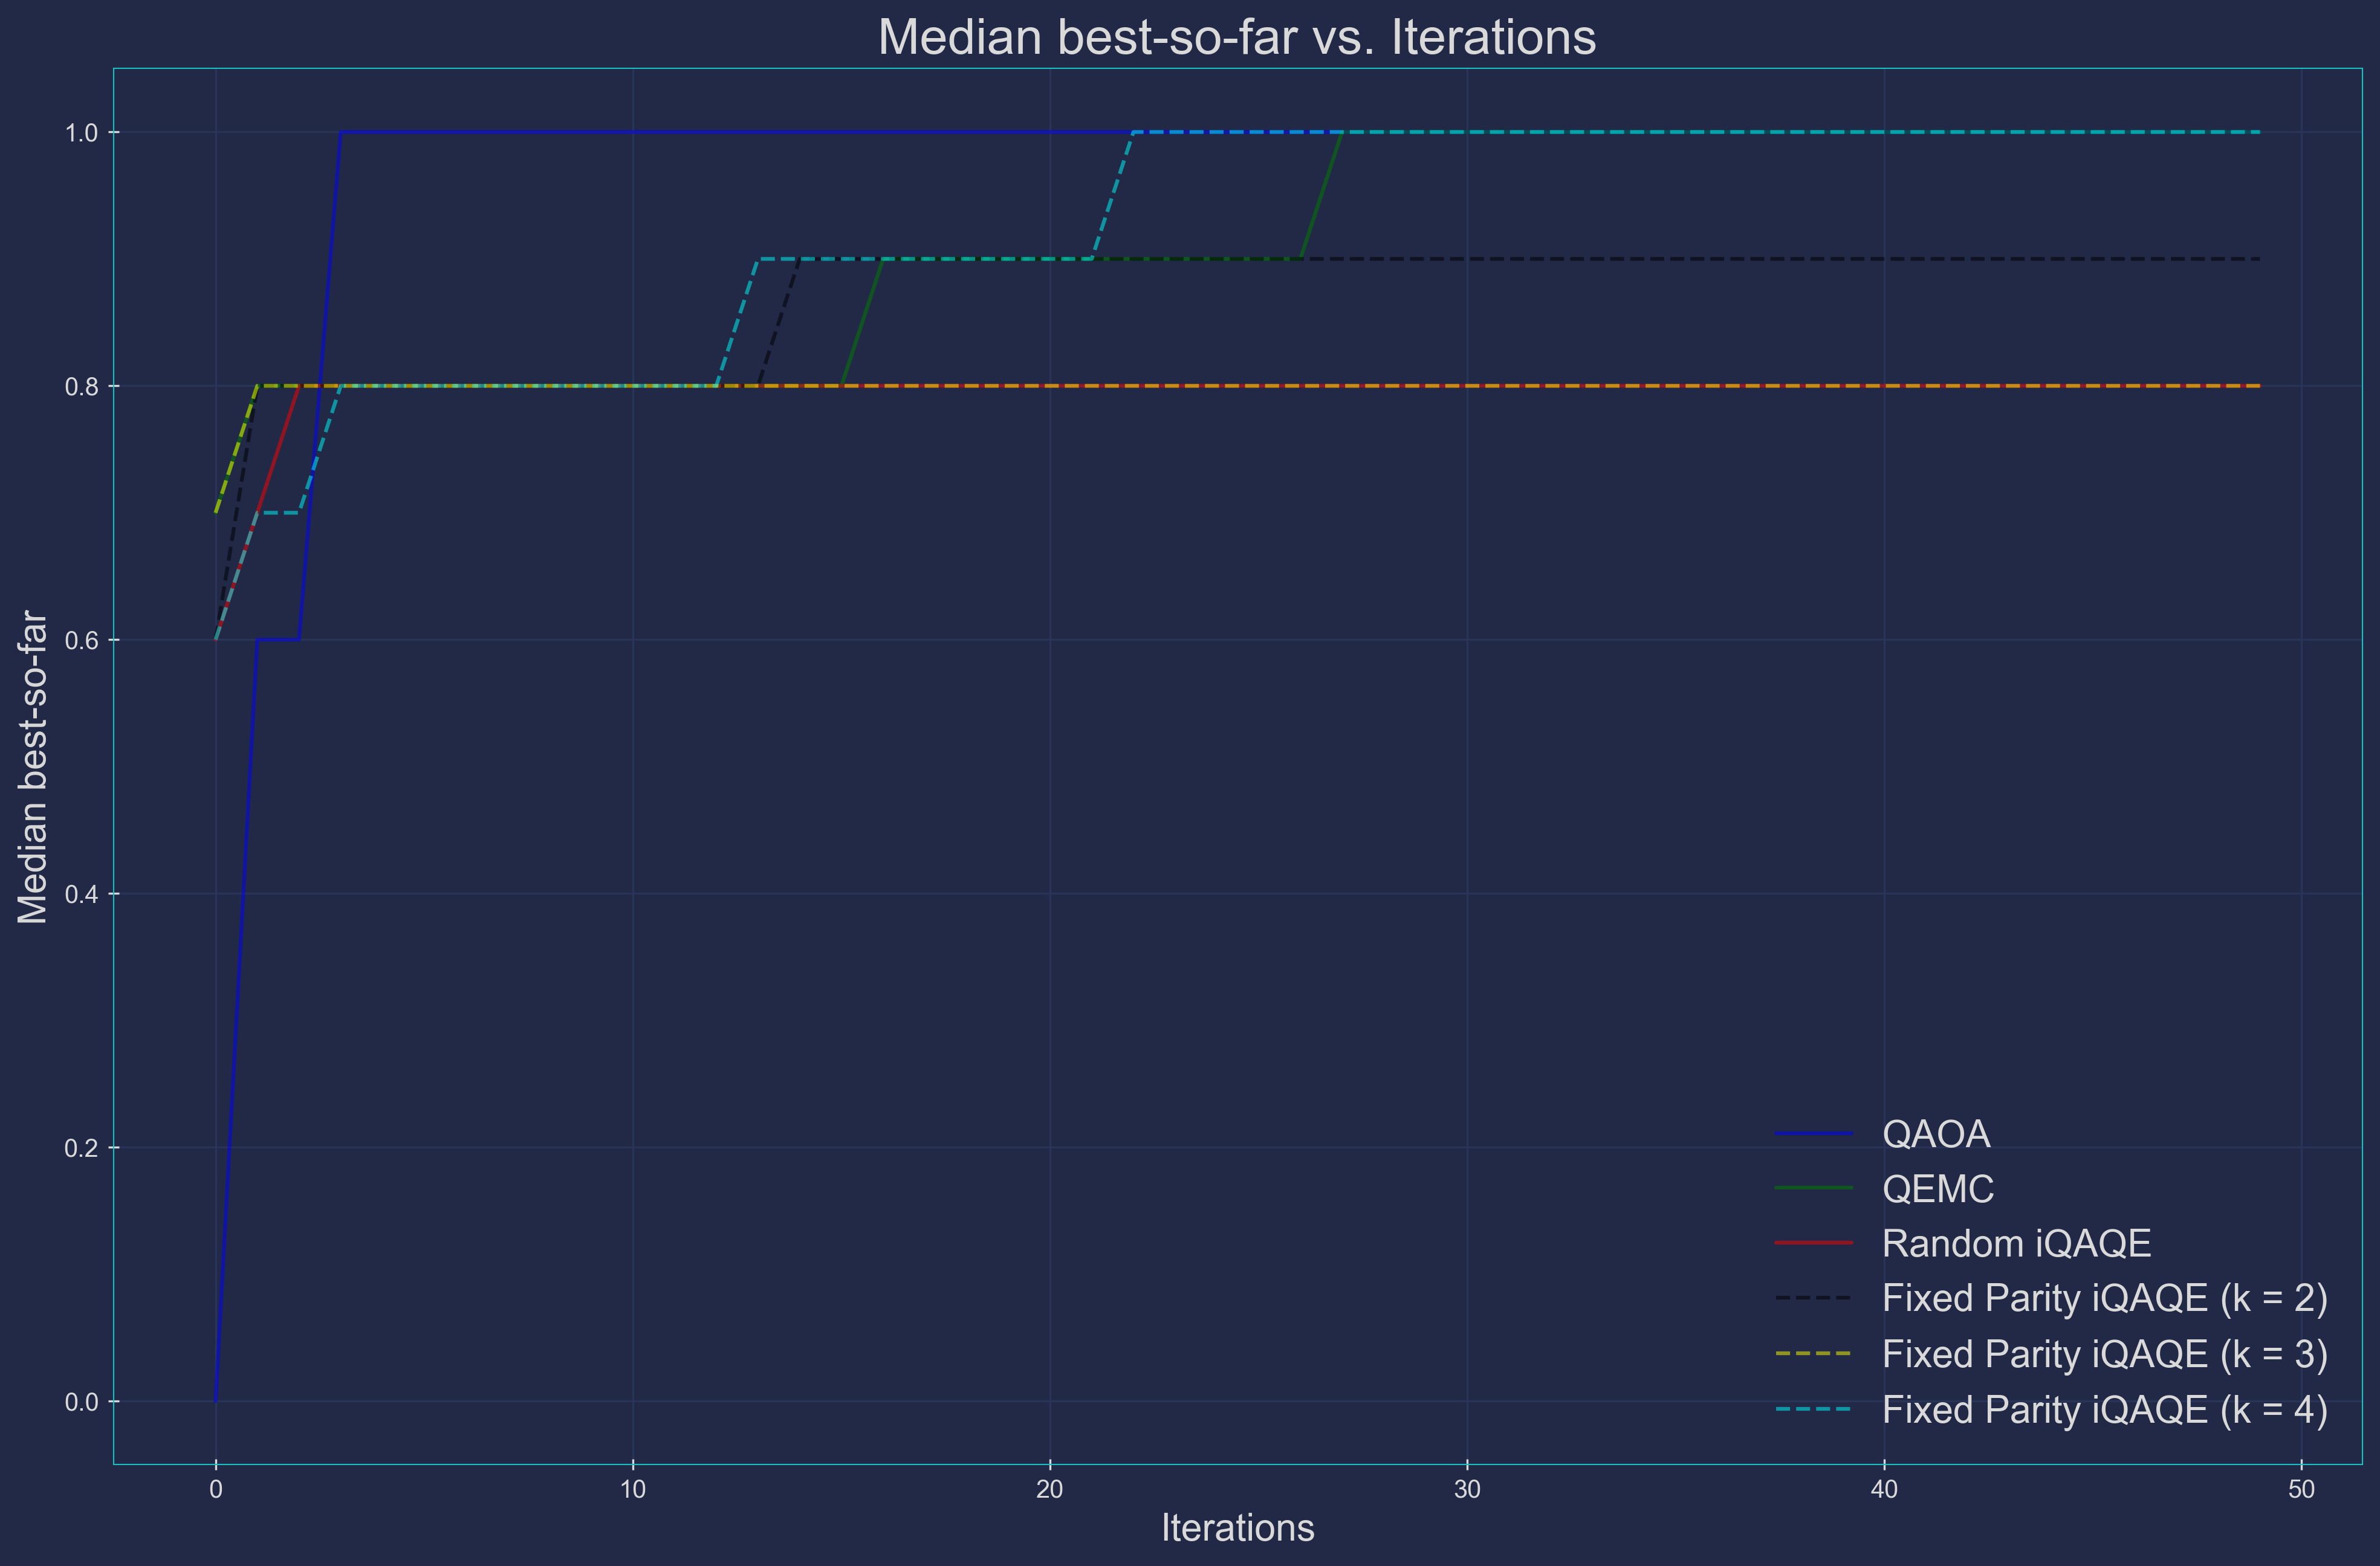
\includegraphics[width=0.975\textwidth]{Figures/Appendix_A/8-node/Basic+Fixed_Parity_iQAQE(8-node).png}
        \caption{\raggedright Fixed-parity scheme compared to \acrshort{qaoa}, \acrshort{qemc}, and a randomly chosen \acrshort{iqaqe} instance.}
        \label{fig:C_BSF_2_8-node}
    \end{subfigure}
    
    \bigskip

    \begin{subfigure}[t]{0.495\textwidth}
        \centering
        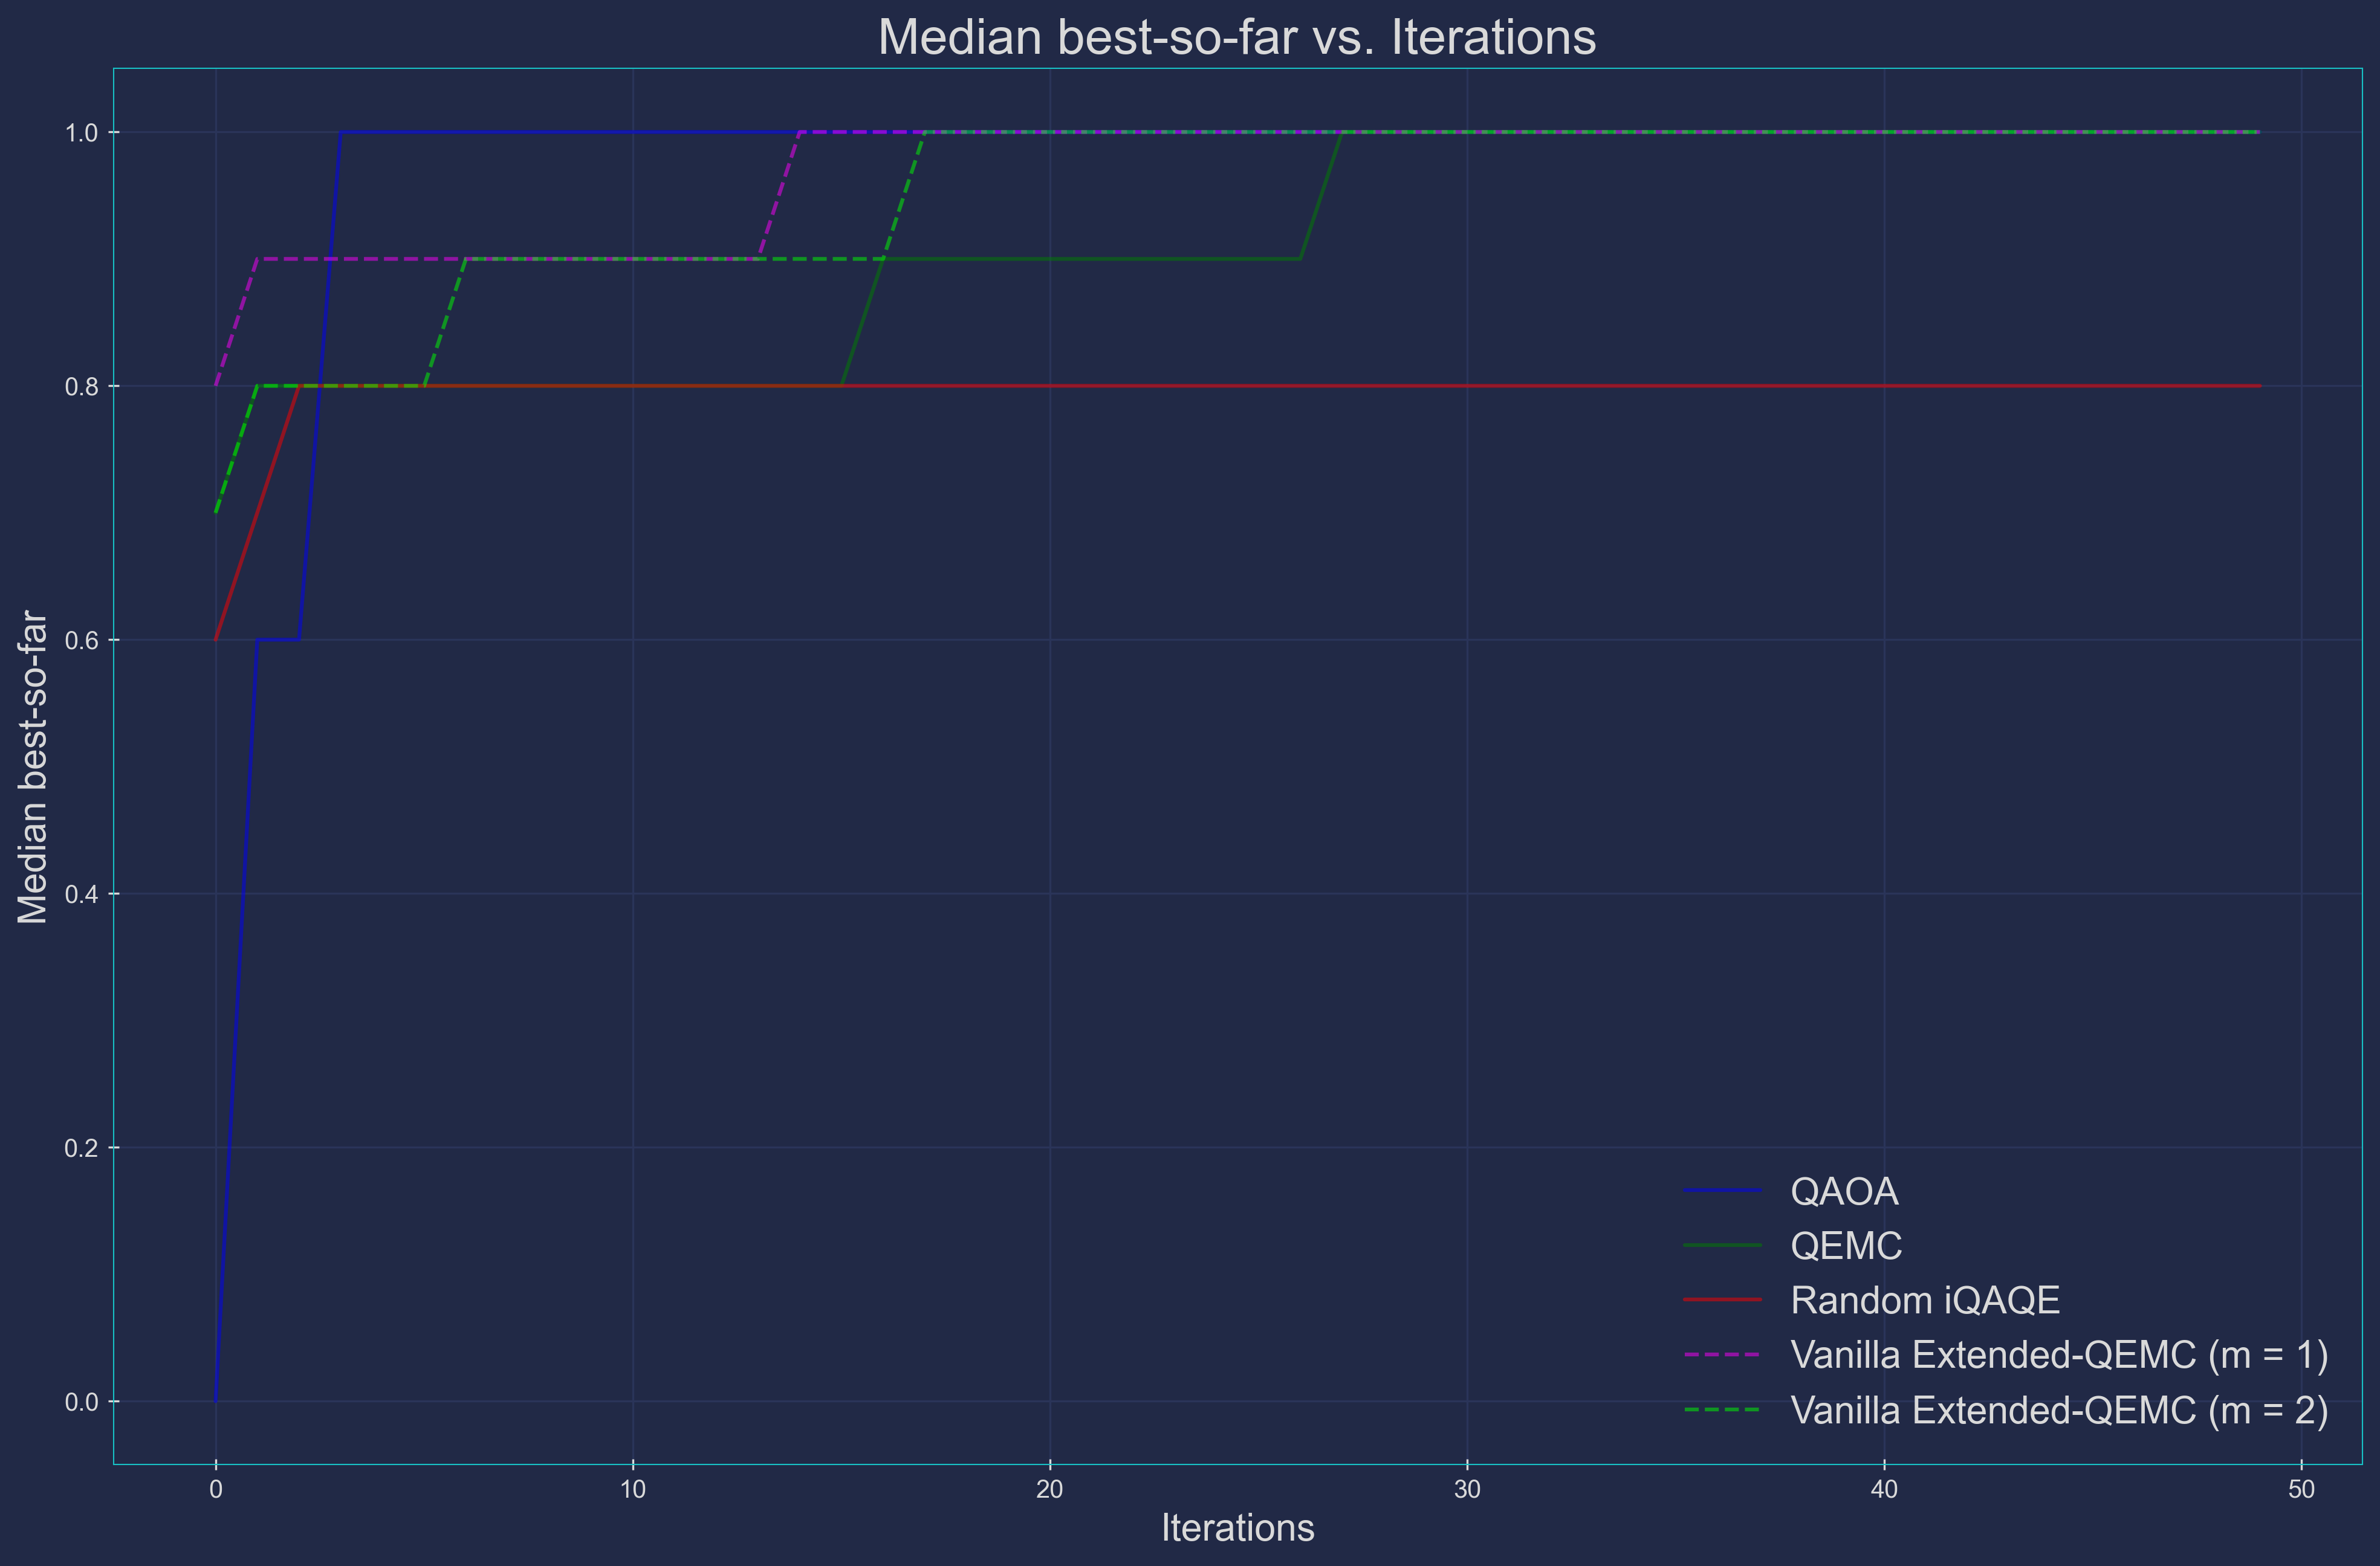
\includegraphics[width=0.975\textwidth]{Figures/Appendix_A/8-node/Basic+V_Extended_QEMC(8-node).png}
        \caption{\raggedright Unmodified (Vanilla) Extended-QEMC scheme compared to \acrshort{qaoa}, \acrshort{qemc}, and a randomly chosen \acrshort{iqaqe} instance.}
        \label{fig:C_BSF_3_8-node}
    \end{subfigure}
    \hfill
    \begin{subfigure}[t]{0.495\textwidth}
        \centering
        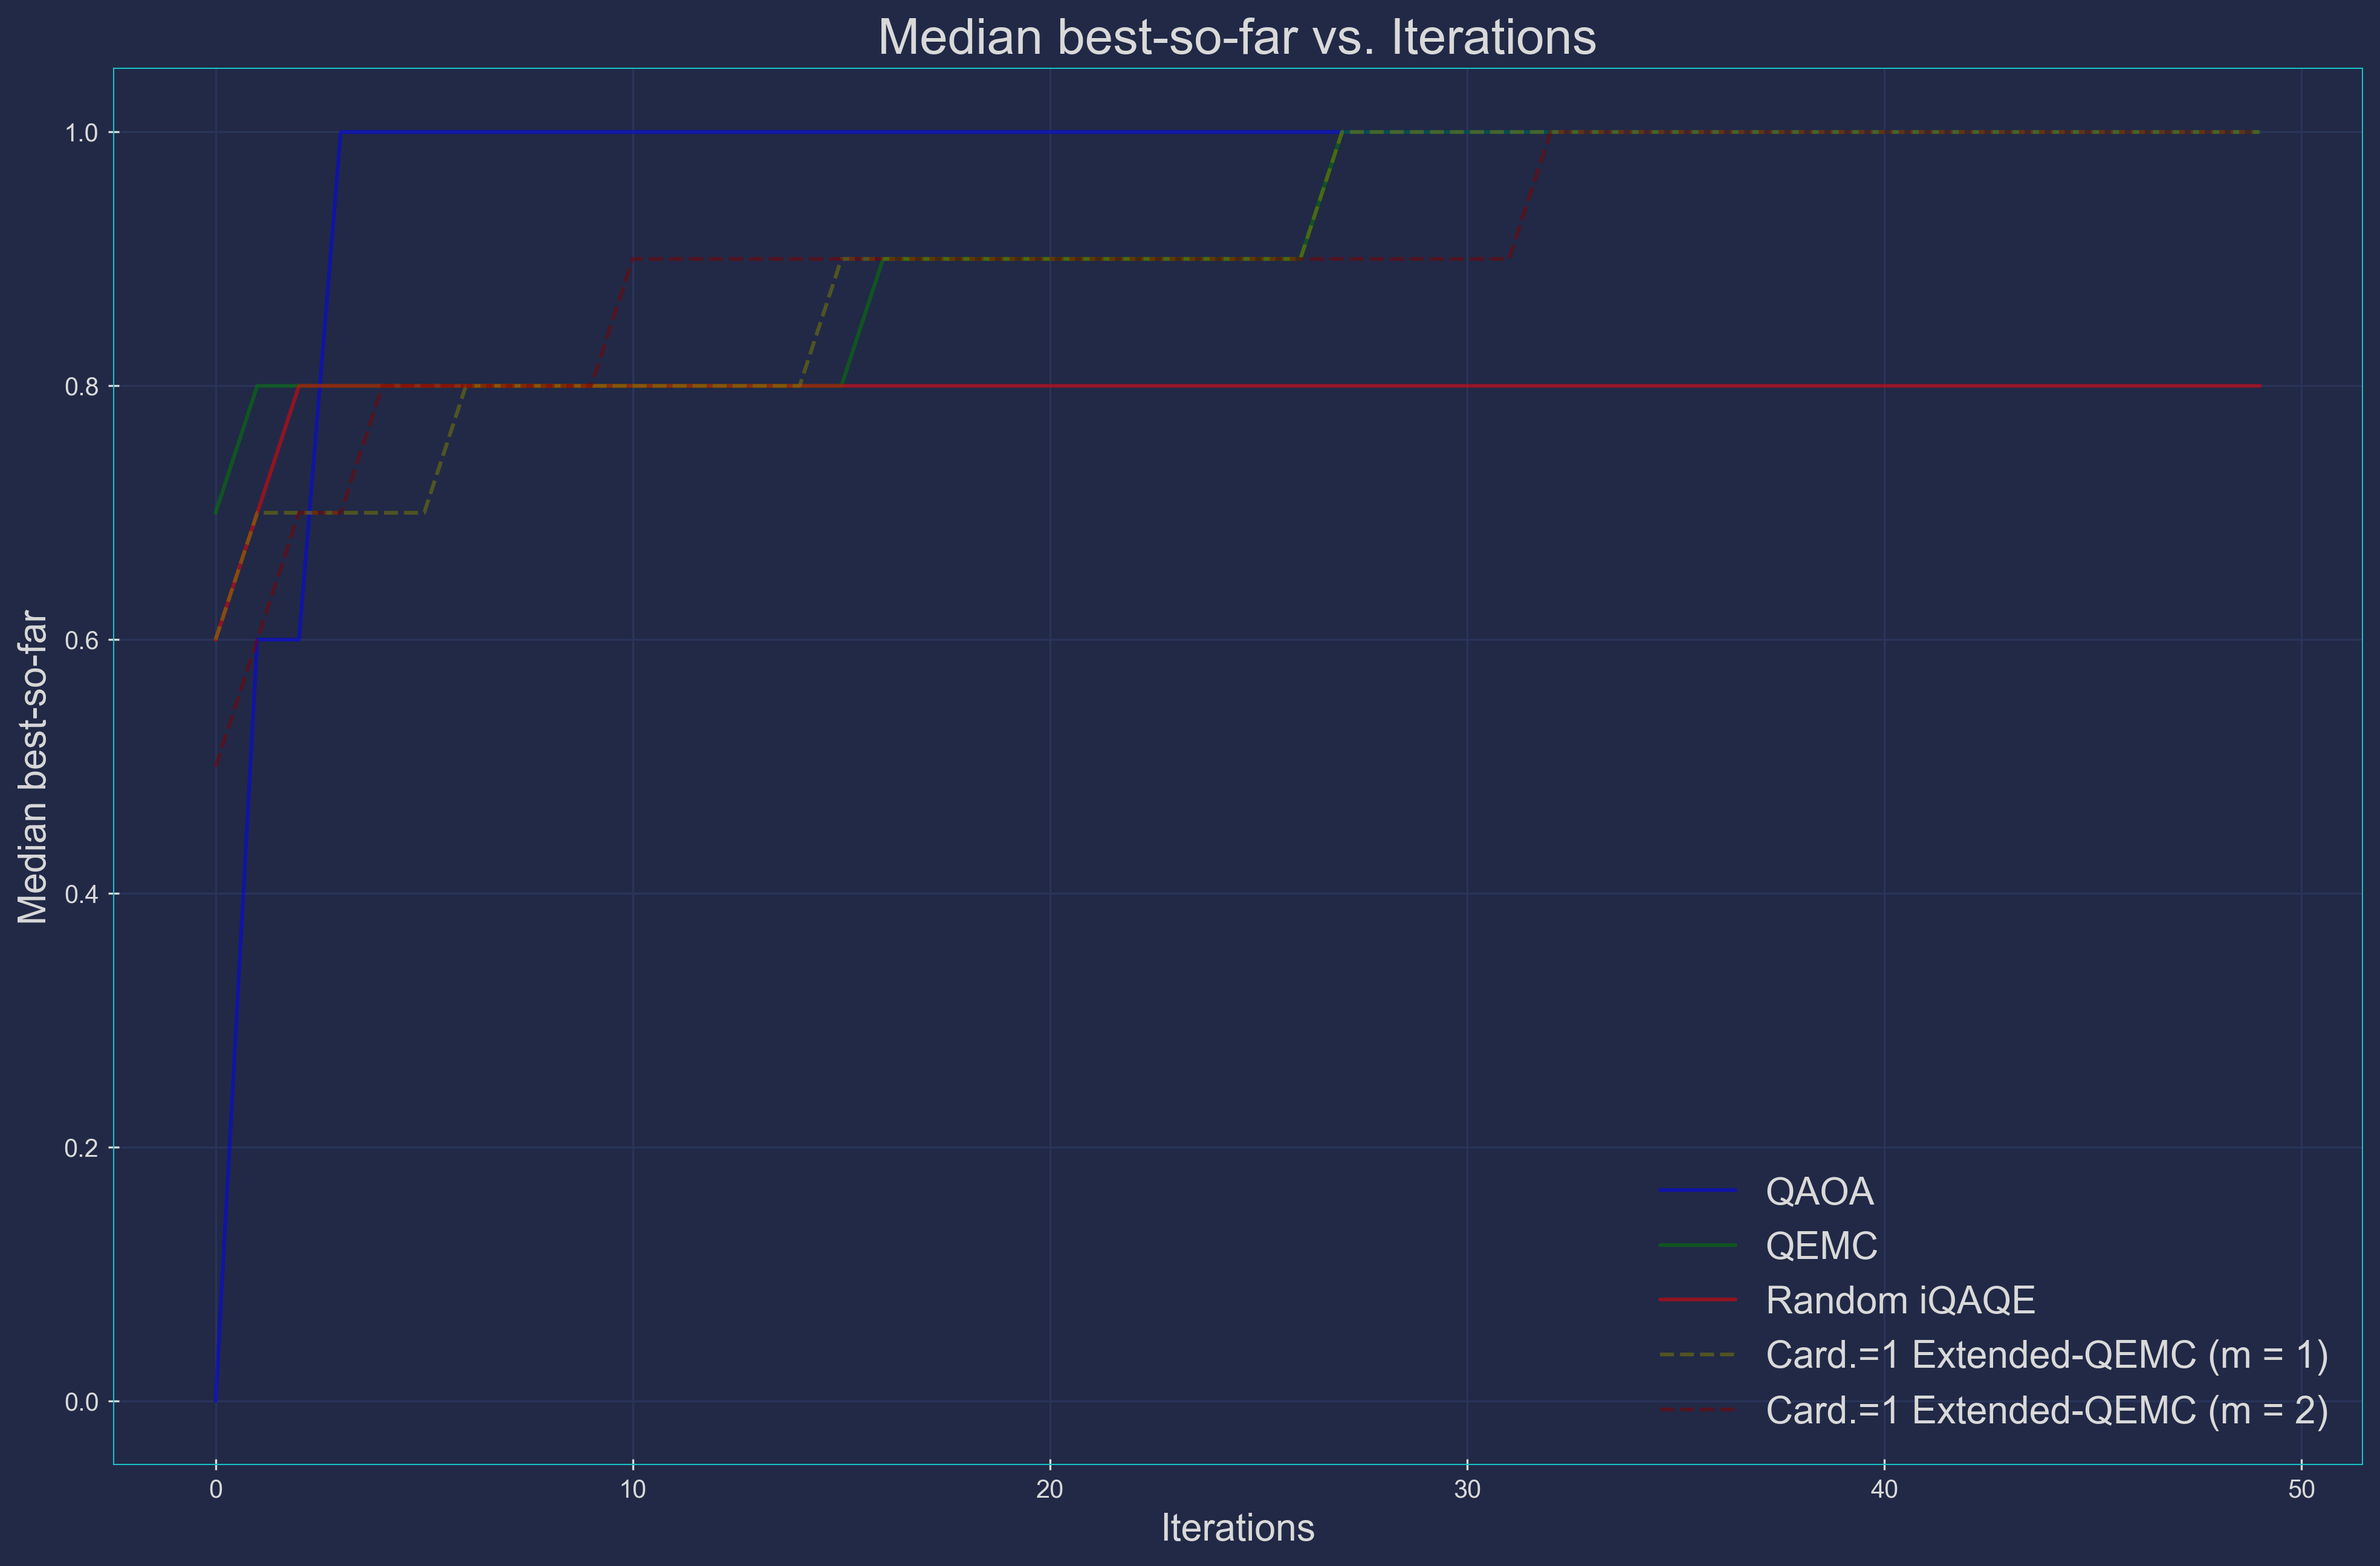
\includegraphics[width=0.975\textwidth]{Figures/Appendix_A/8-node/Basic+C1_Extended_QEMC(8-node).png}
        \caption{\raggedright Cardinality $= 1$ Extended-QEMC scheme compared to \acrshort{qaoa}, \acrshort{qemc}, and a randomly chosen \acrshort{iqaqe} instance.}
        \label{fig:C_BSF_4_8-node}
    \end{subfigure}

    \bigskip

    \centering
    \begin{subfigure}[t]{0.90\textwidth}
		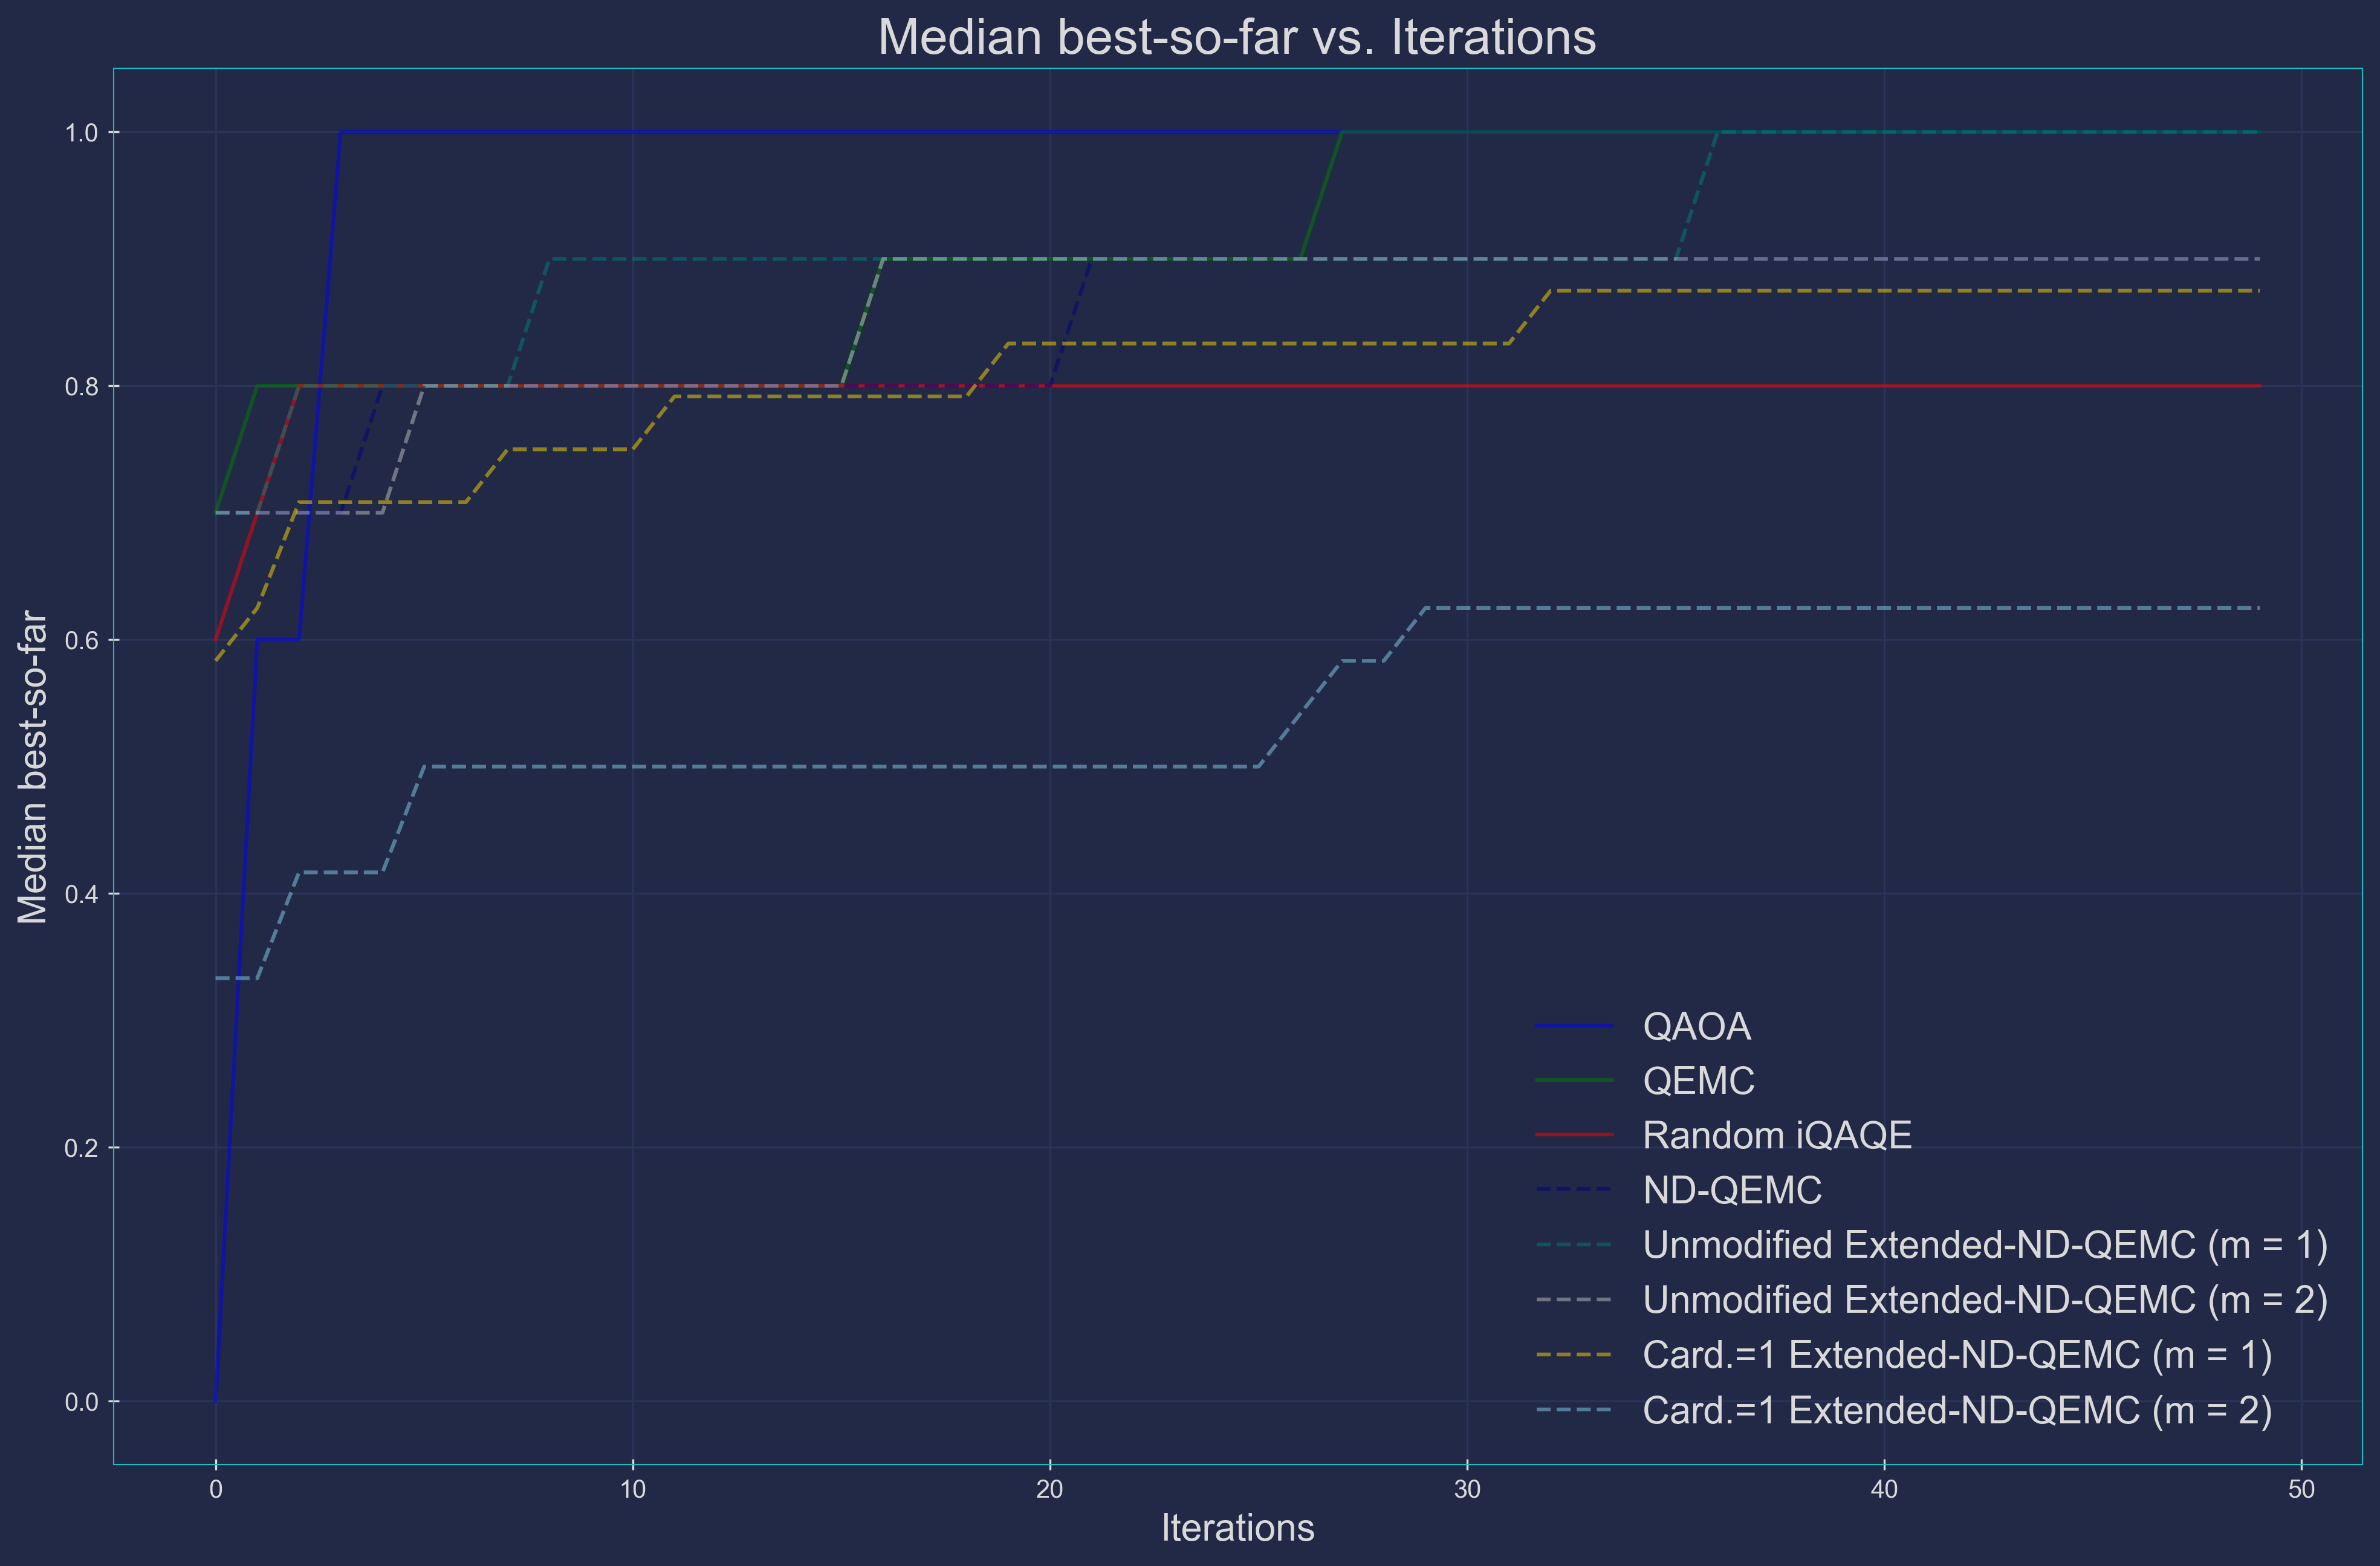
\includegraphics[width=1\textwidth]{Figures/Appendix_A/8-node/Basic+ND_QEMC_Variations(8-node).png}
		\caption{\raggedright Non-deterministic CNOT-gate-using schemes compared to \acrshort{qaoa}, \acrshort{qemc}, and a randomly chosen \acrshort{iqaqe} instance.}
		\label{fig:C_BSF_5_8-node}
	\end{subfigure}

    \caption{Revised results using the median best-so-far \acrshort{ar} metric for the $8$-node graph.}
    \label{fig:Corrected_BSF_Results_32&100-node}
\end{figure*}

%%%%%%%%%%%%%%%%%%%%%%%%%%%%%%%%%%%%%%%%%%%%%%%%%%%%%%%%%%%%%%%%%%%%%%%%%%%%%%%%%%%%%%%%%%%%%%%%%%%%%%%

% % This is what I had before fixing the plots to be: 4-5. I had 5-4 before.

% \begin{figure*}[hb!]
%     \centering
%     \begin{subfigure}[t]{0.495\textwidth}
%         \centering
%         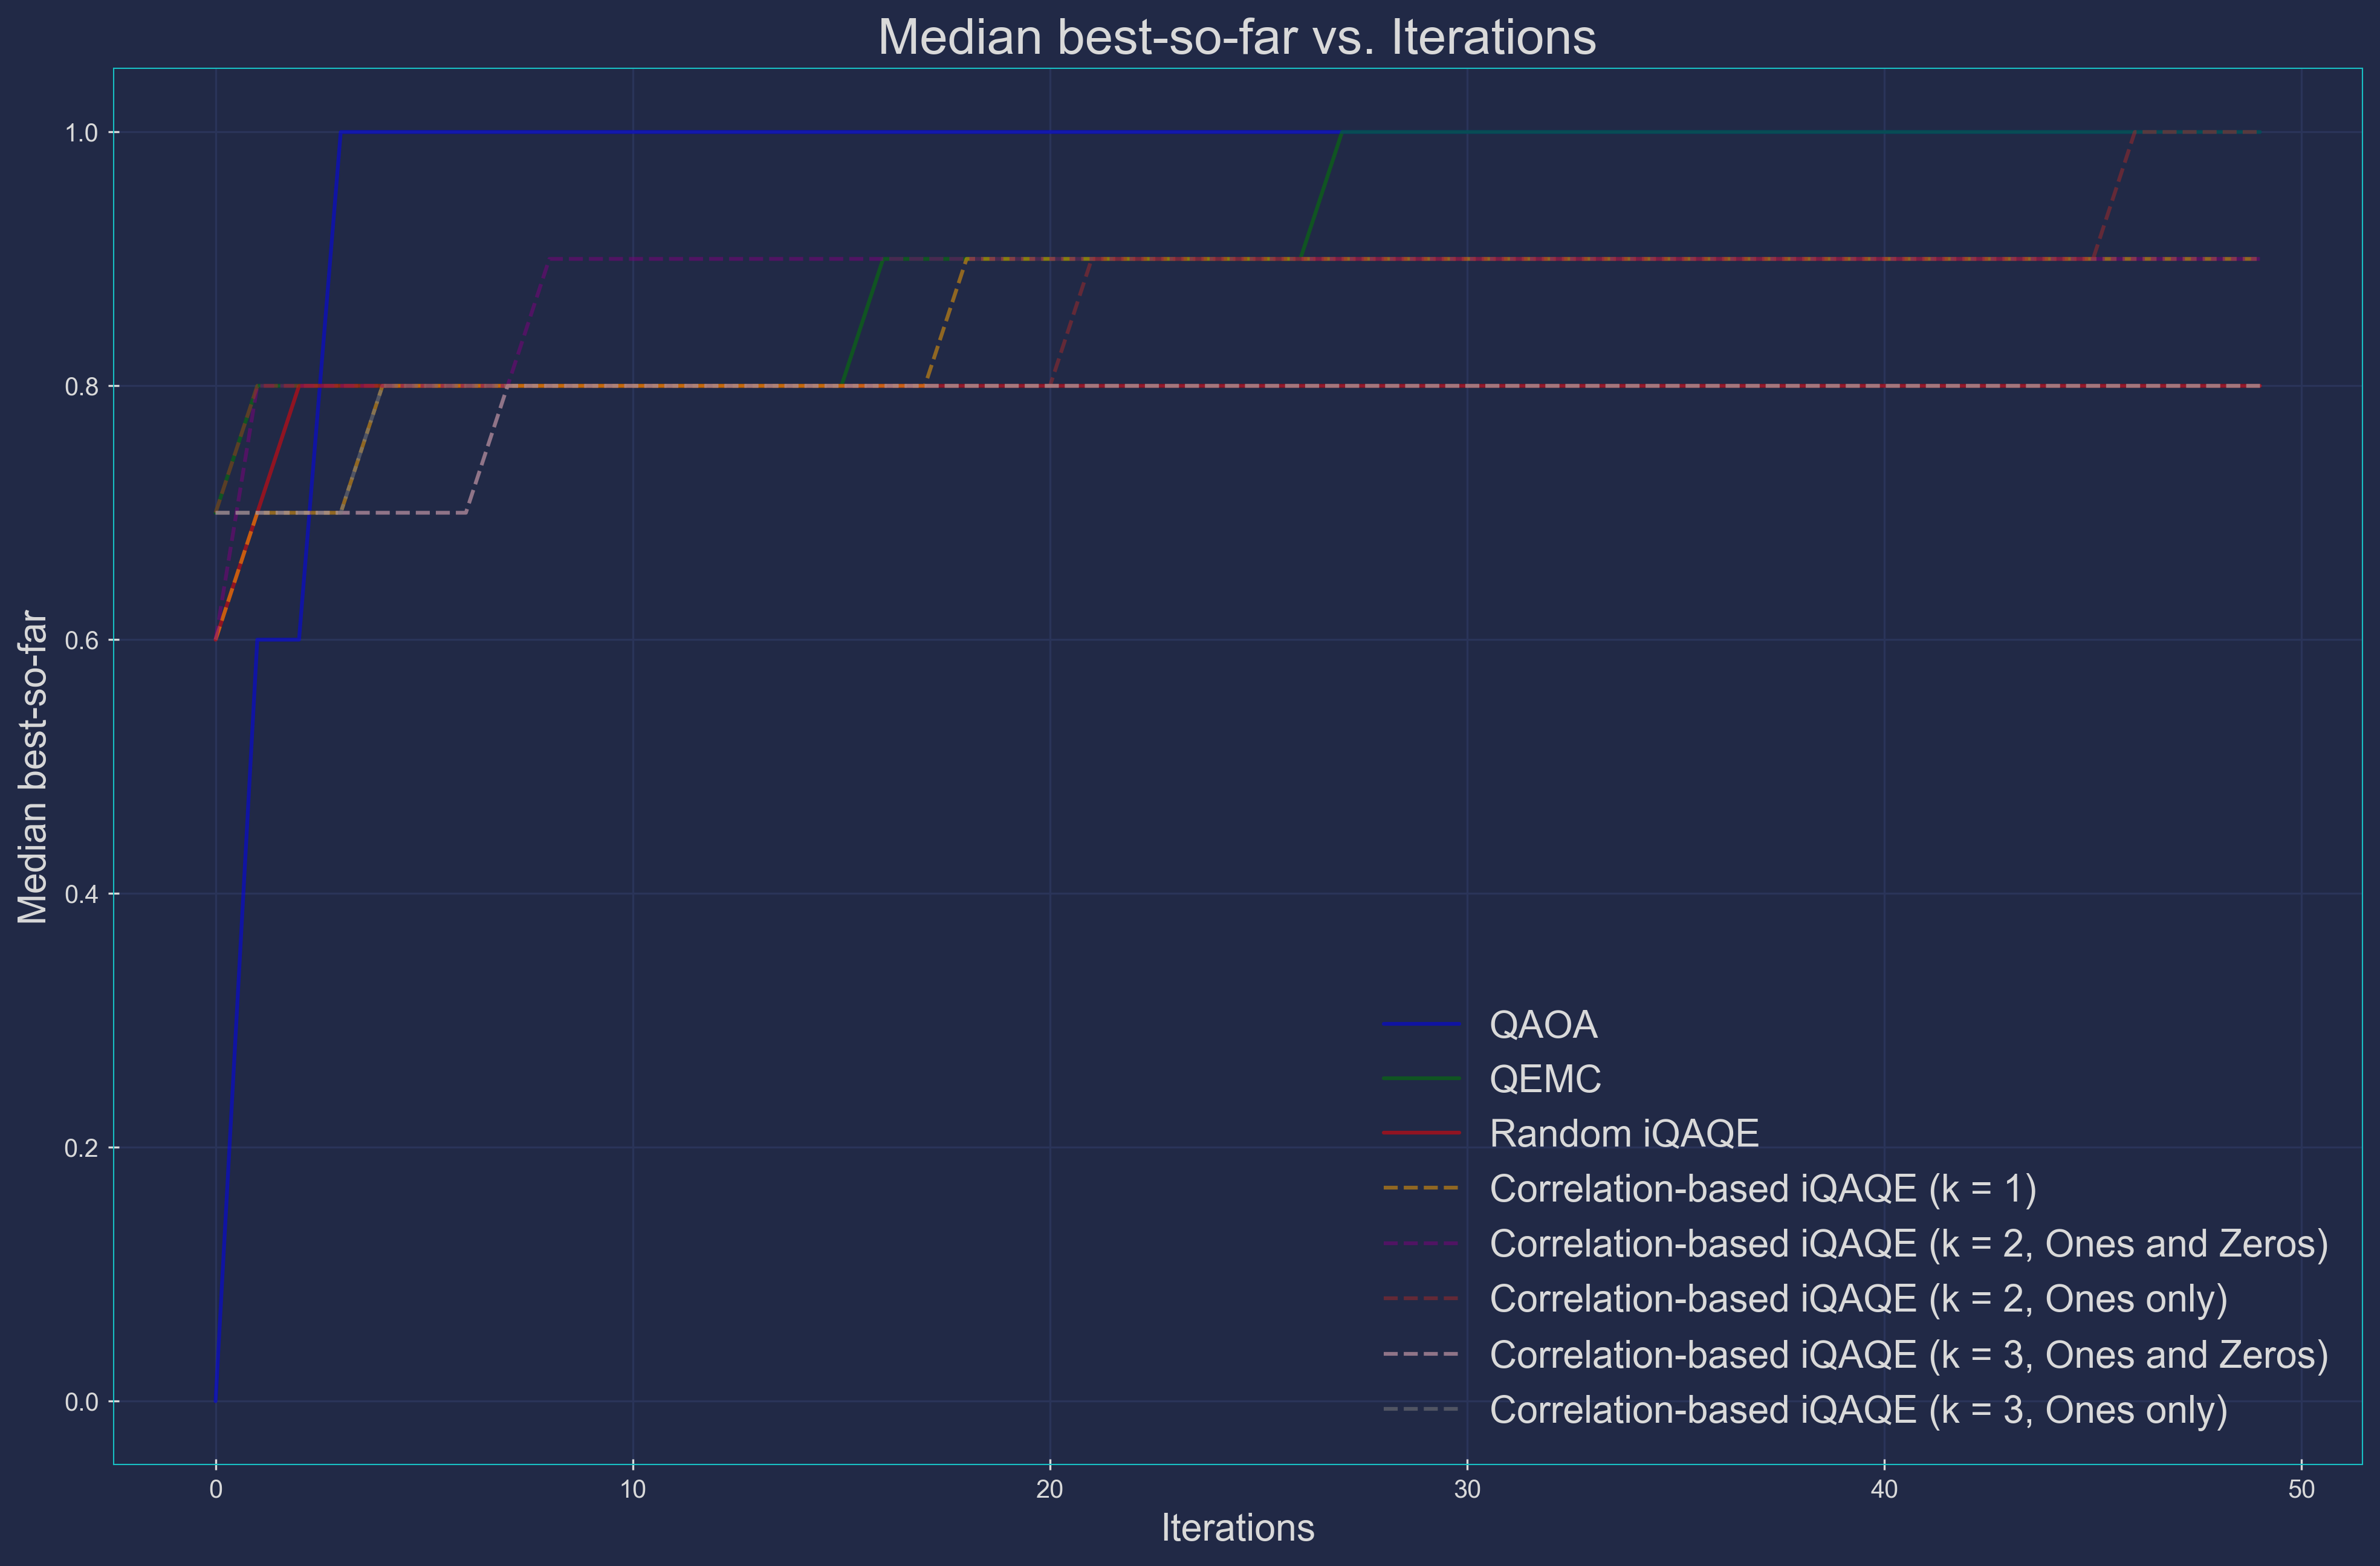
\includegraphics[width=1\textwidth, height=0.656\textwidth]{Figures/Appendix_A/8-node/Basic+Correlation_iQAQE(8-node).png}
%         \caption{\raggedright Correlation-based schemes compared to \acrshort{qaoa}, \acrshort{qemc}, and a randomly chosen \acrshort{iqaqe} instance.}
%         \label{fig:C_BSF_1_8-node}
%     \end{subfigure}
%     \hfill
%     \begin{subfigure}[t]{0.495\textwidth}
%         \centering
%         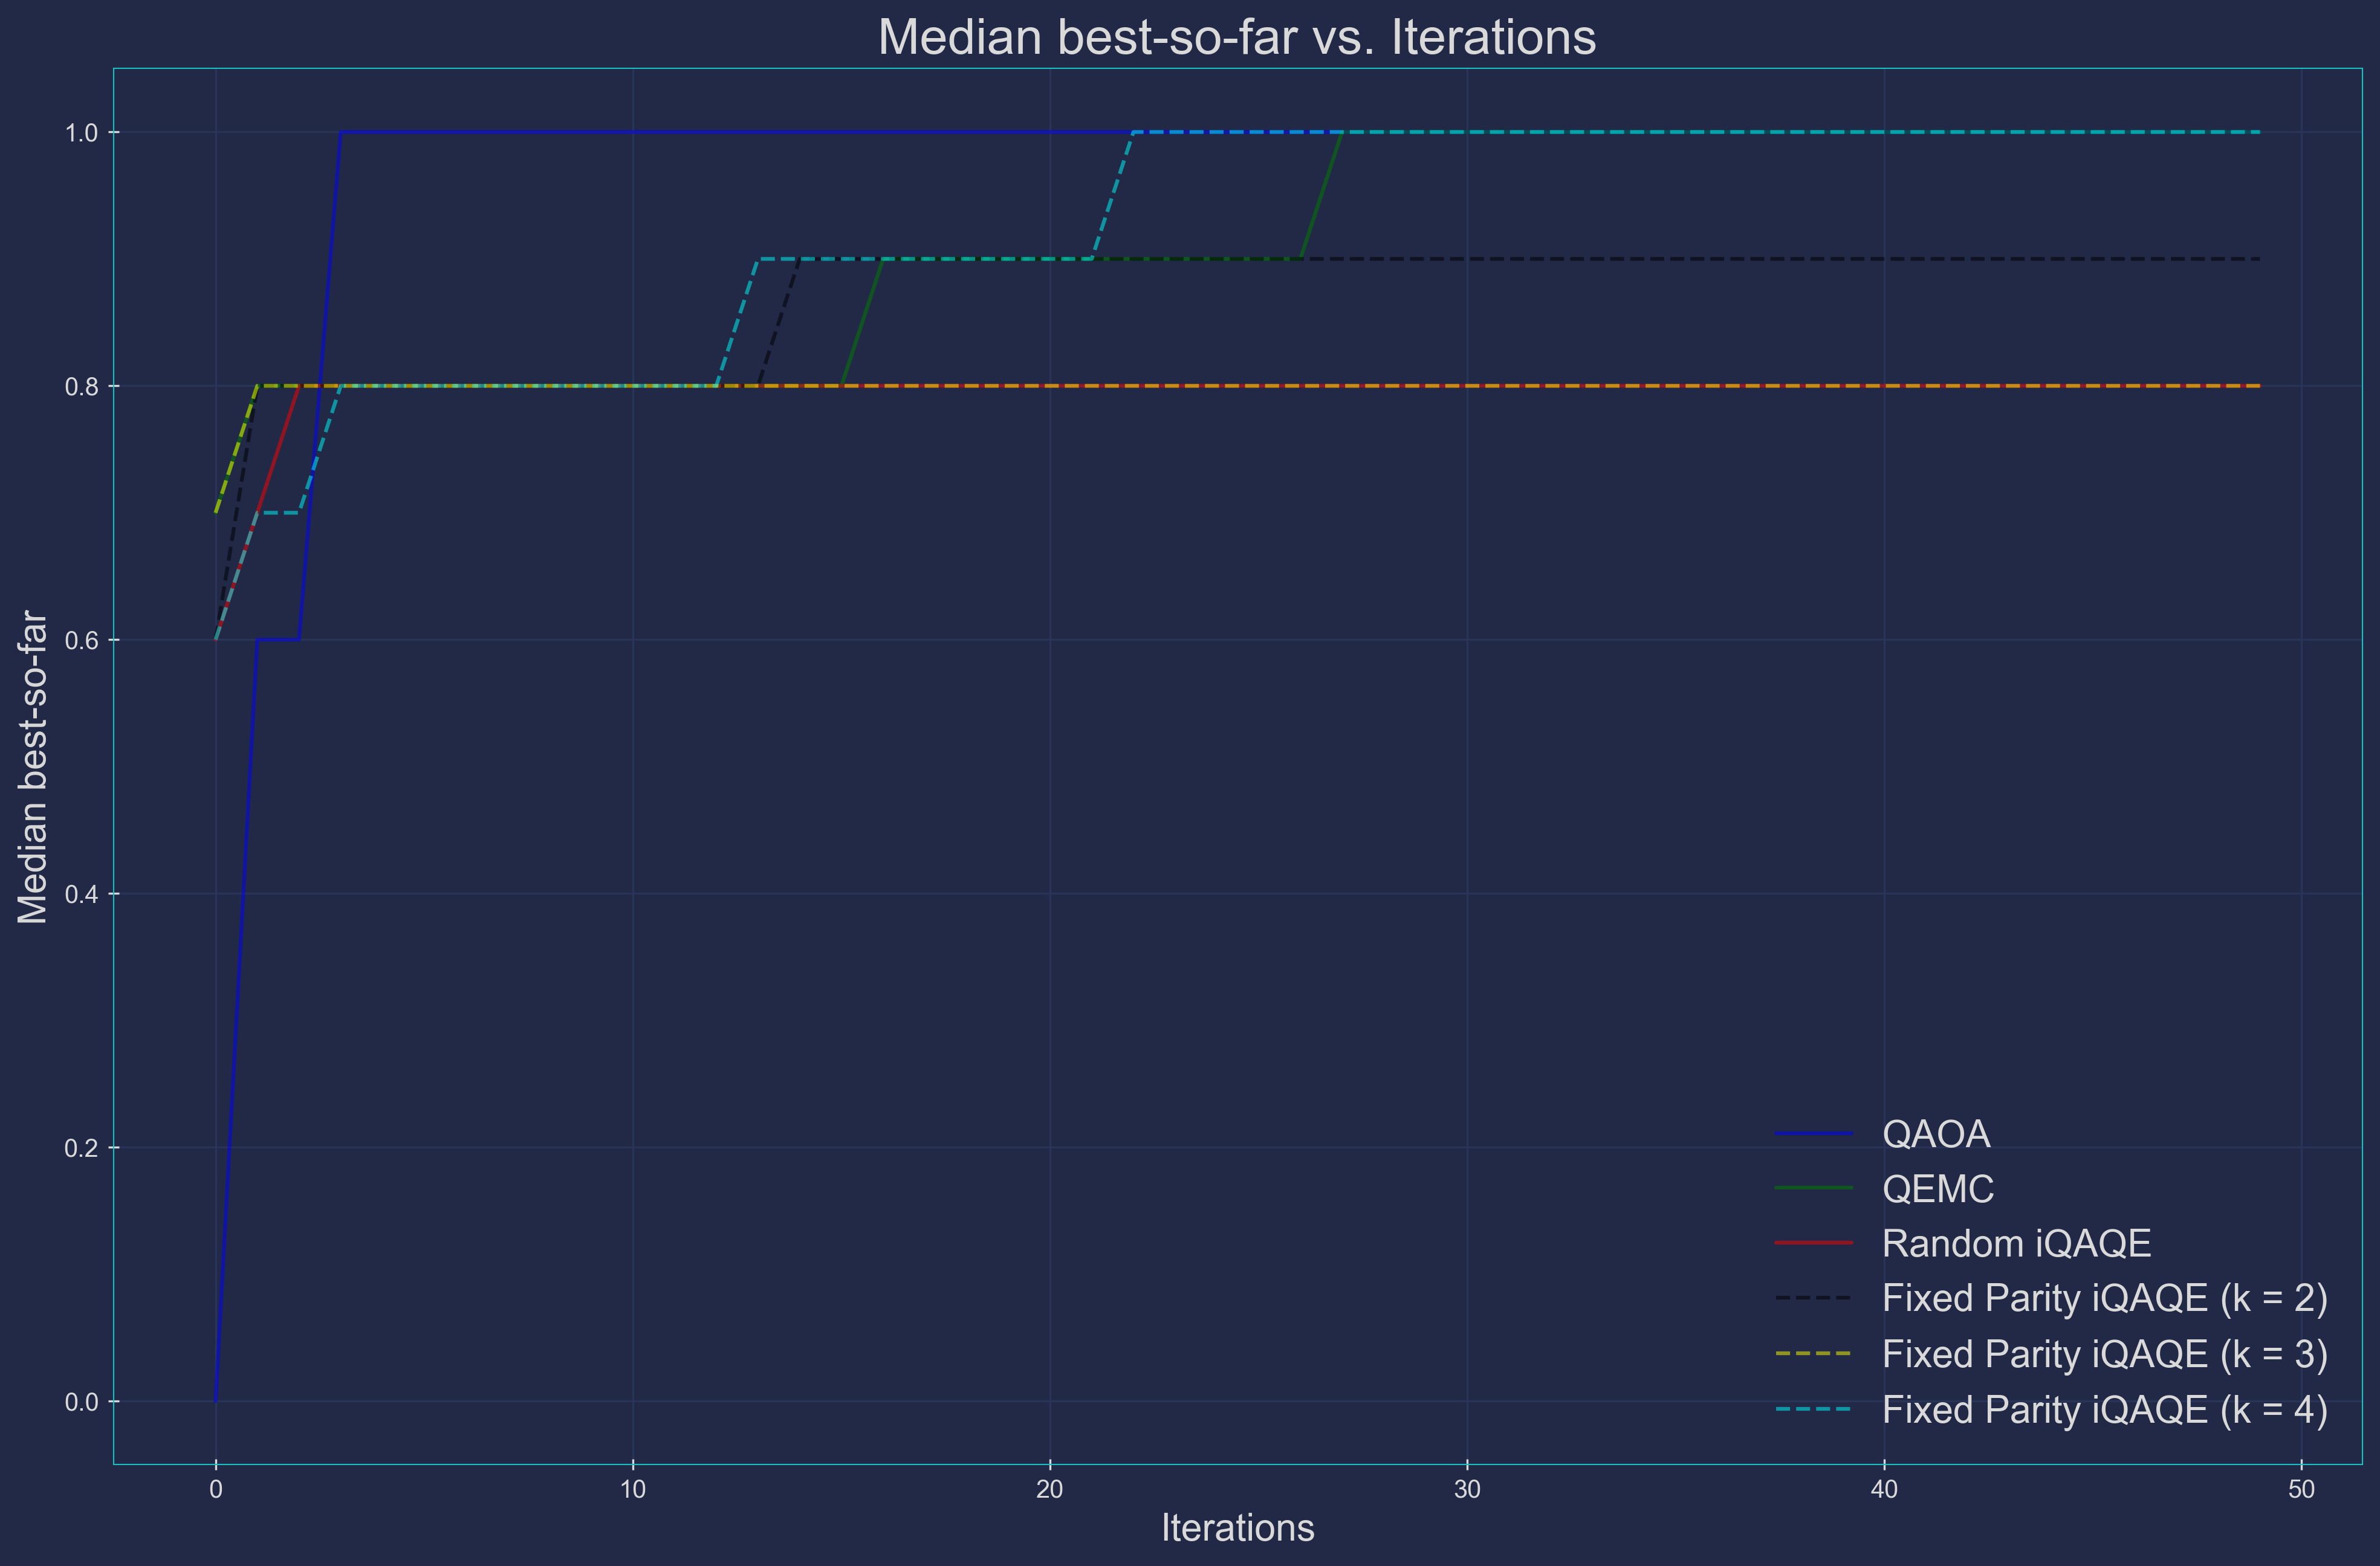
\includegraphics[width=1\textwidth, height=0.656\textwidth]{Figures/Appendix_A/8-node/Basic+Fixed_Parity_iQAQE(8-node).png}
%         \caption{Fixed-parity scheme compared to \acrshort{qaoa}, \acrshort{qemc}, and a randomly chosen \acrshort{iqaqe} instance.}
%         \label{fig:C_BSF_2_8-node}
%     \end{subfigure}
% \end{figure*}

% \begin{figure*}[ht!]
%     \addtocounter{figure}{-1} % Added <<
%     \centering
%     \begin{subfigure}[t]{0.495\textwidth}
%         \addtocounter{subfigure}{2} % Added <<
%         \centering
%         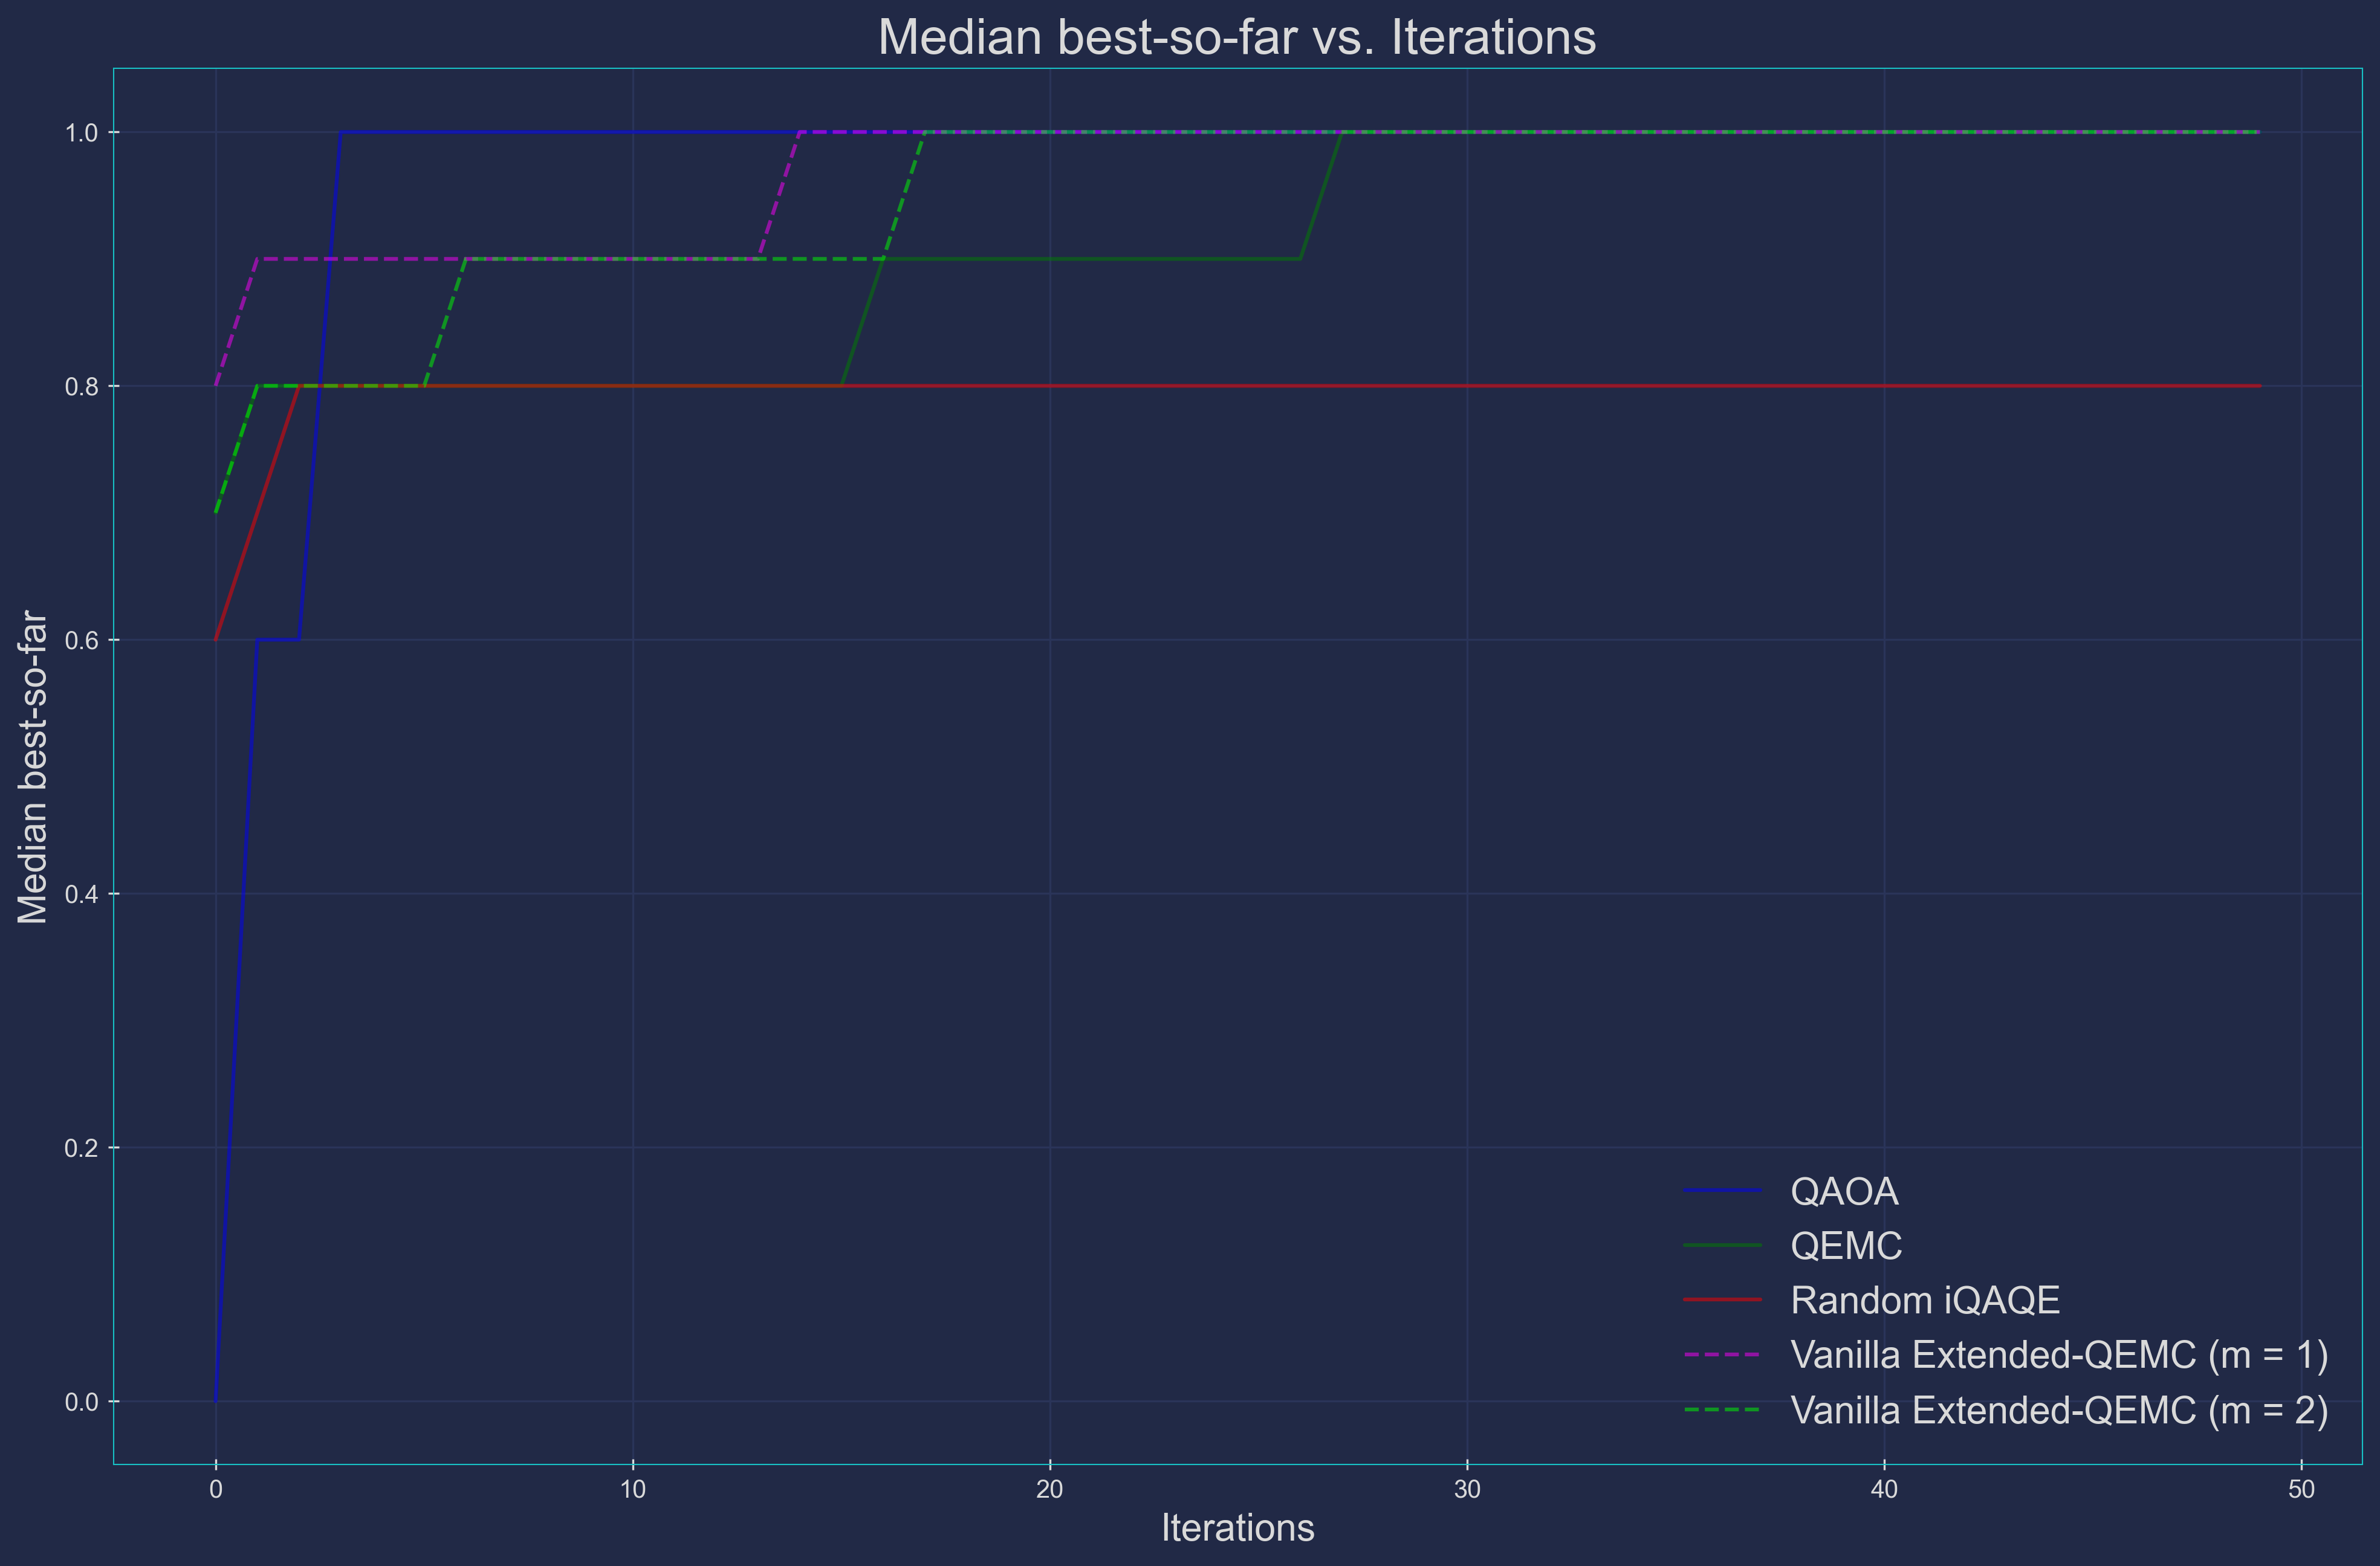
\includegraphics[width=1\textwidth, height=0.656\textwidth]{Figures/Appendix_A/8-node/Basic+V_Extended_QEMC(8-node).png}
%         \caption{Unmodified (Vanilla) Extended-QEMC scheme compared to \acrshort{qaoa}, \acrshort{qemc}, and a randomly chosen \acrshort{iqaqe} instance.}
%         \label{fig:C_BSF_3_8-node}
%     \end{subfigure}
%     \hfill
%     \begin{subfigure}[t]{0.495\textwidth}
%         \centering
%         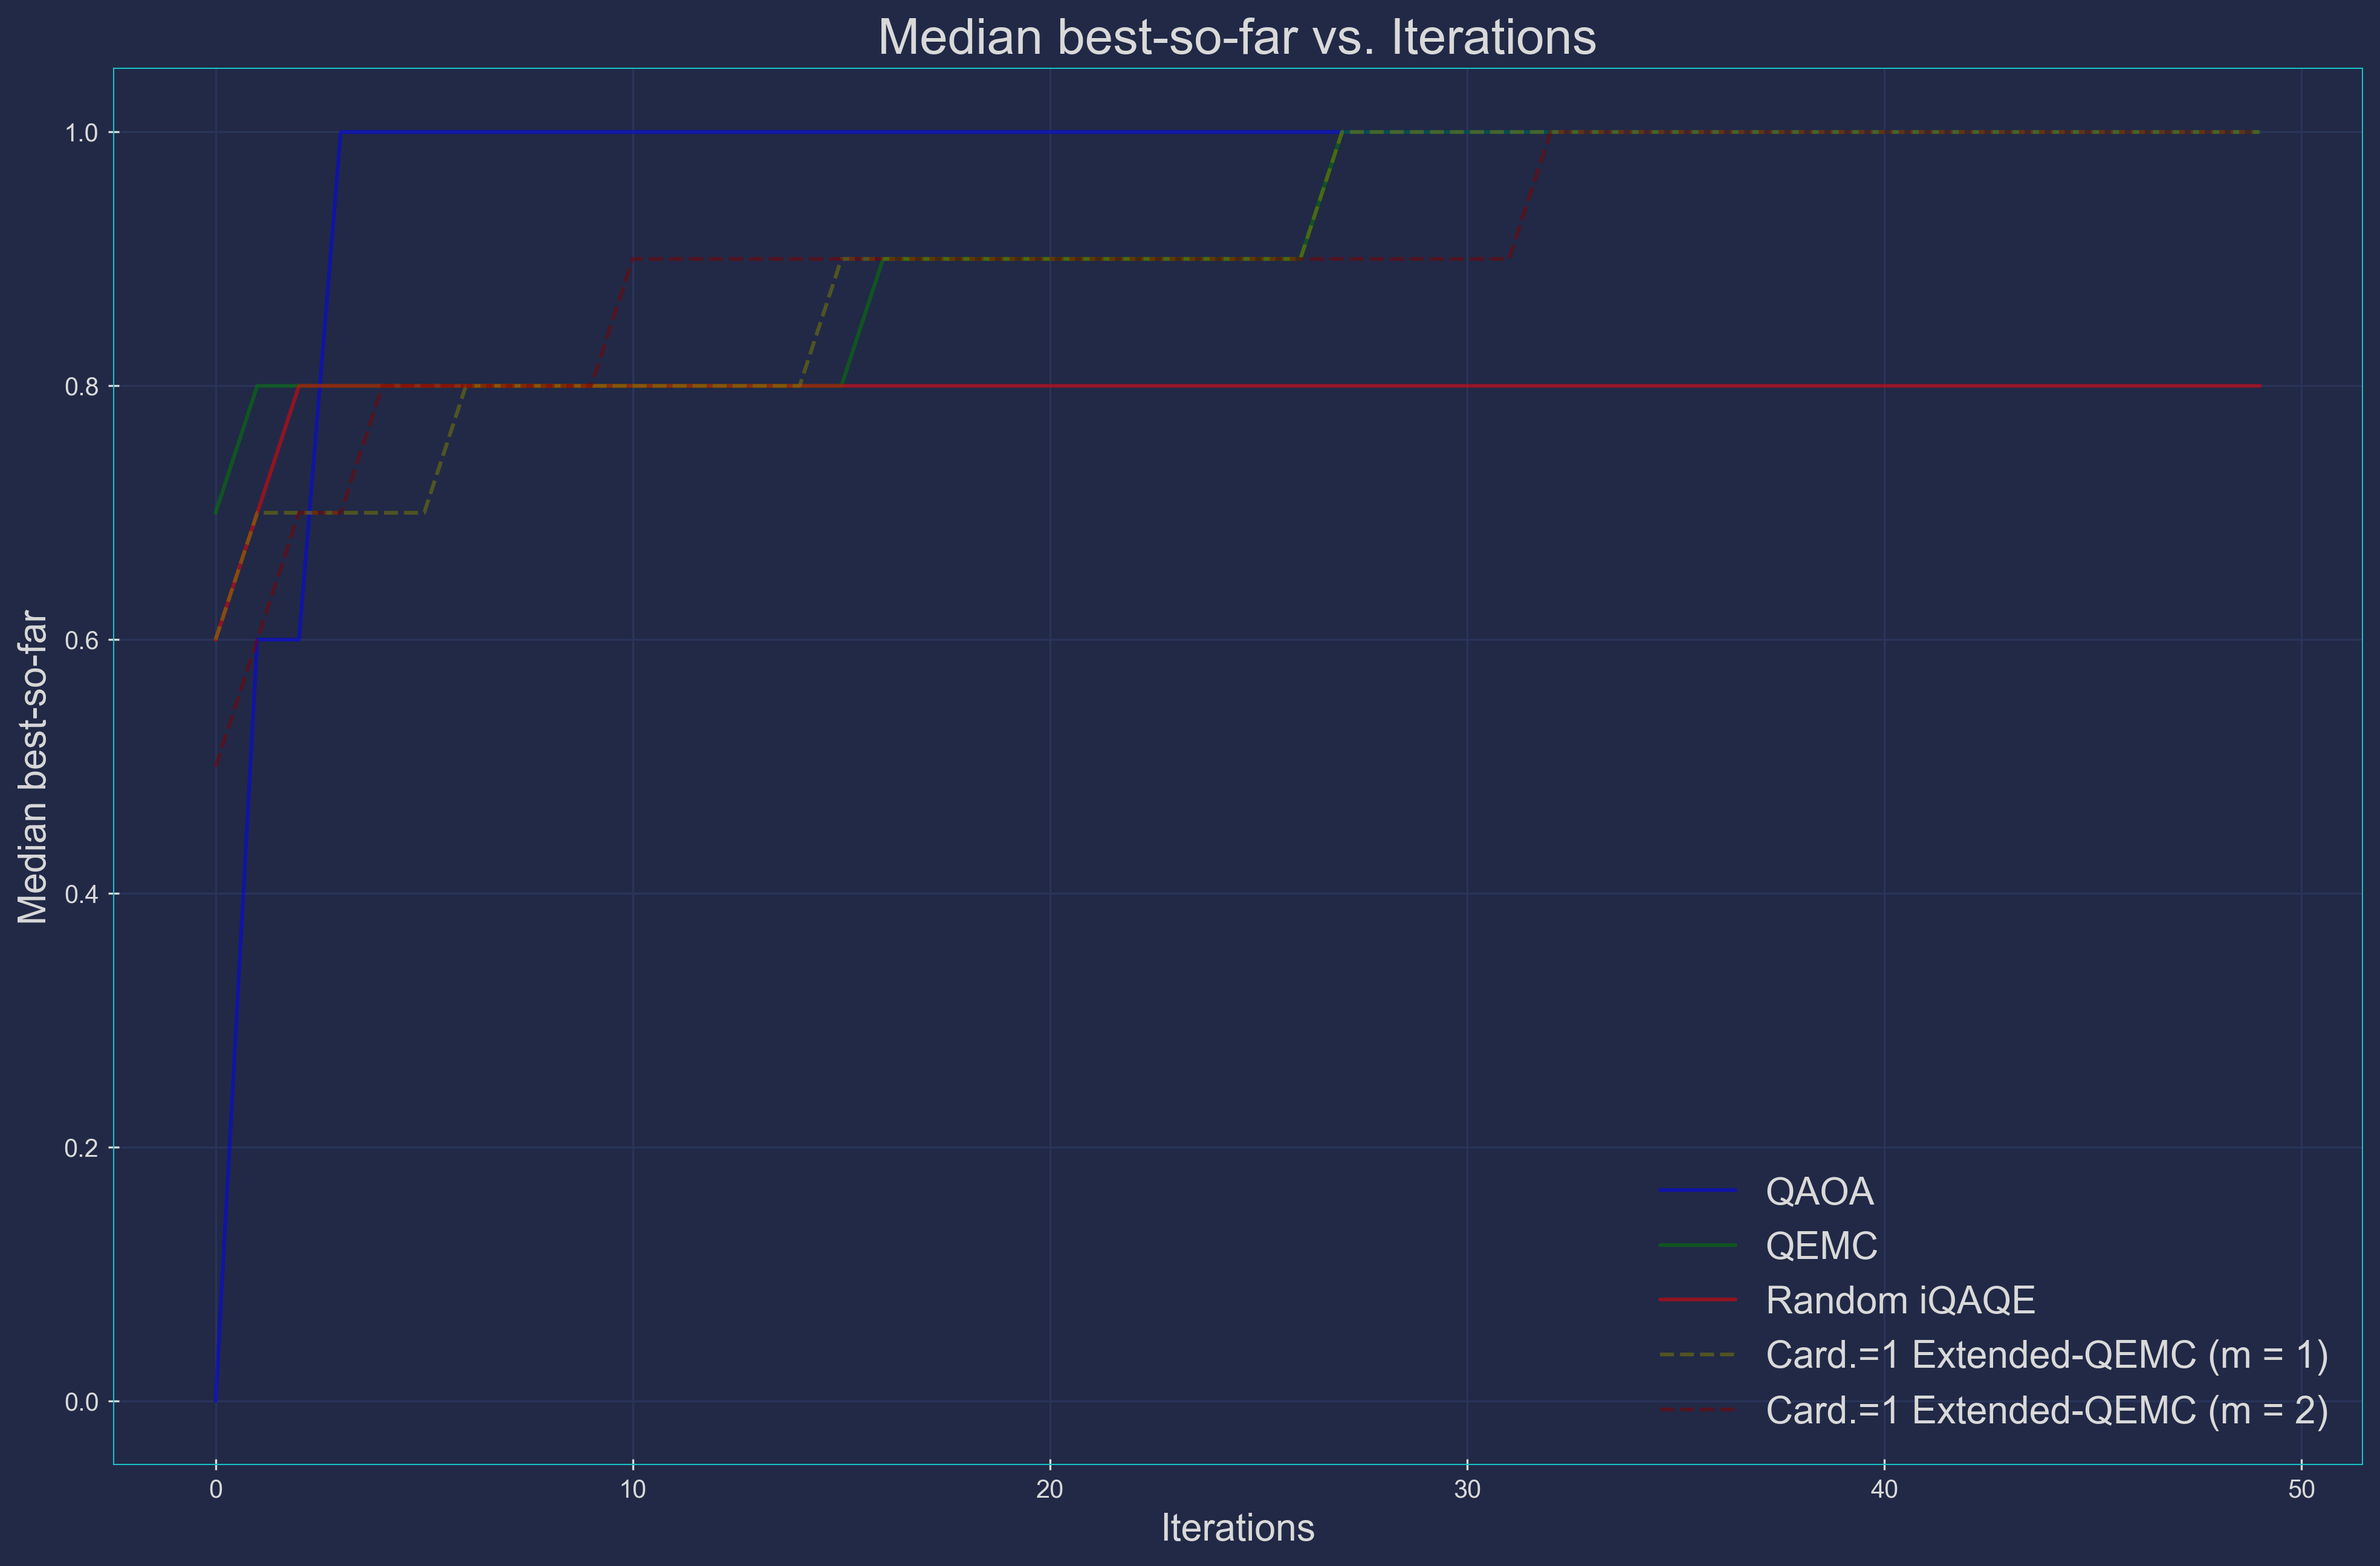
\includegraphics[width=1\textwidth, height=0.656\textwidth]{Figures/Appendix_A/8-node/Basic+C1_Extended_QEMC(8-node).png}
%         \caption{Cardinality $= 1$ Extended-QEMC scheme compared to \acrshort{qaoa}, \acrshort{qemc}, and a randomly chosen \acrshort{iqaqe} instance.}
%         \label{fig:C_BSF_4_8-node}
%     \end{subfigure}
% \end{figure*}

% \clearpage

% \begin{figure*}[ht!]
% 	\addtocounter{figure}{-1} % Added <<
%     \centering
% 	\begin{subfigure}[t]{0.495\textwidth}
% 		\addtocounter{subfigure}{4}
% 		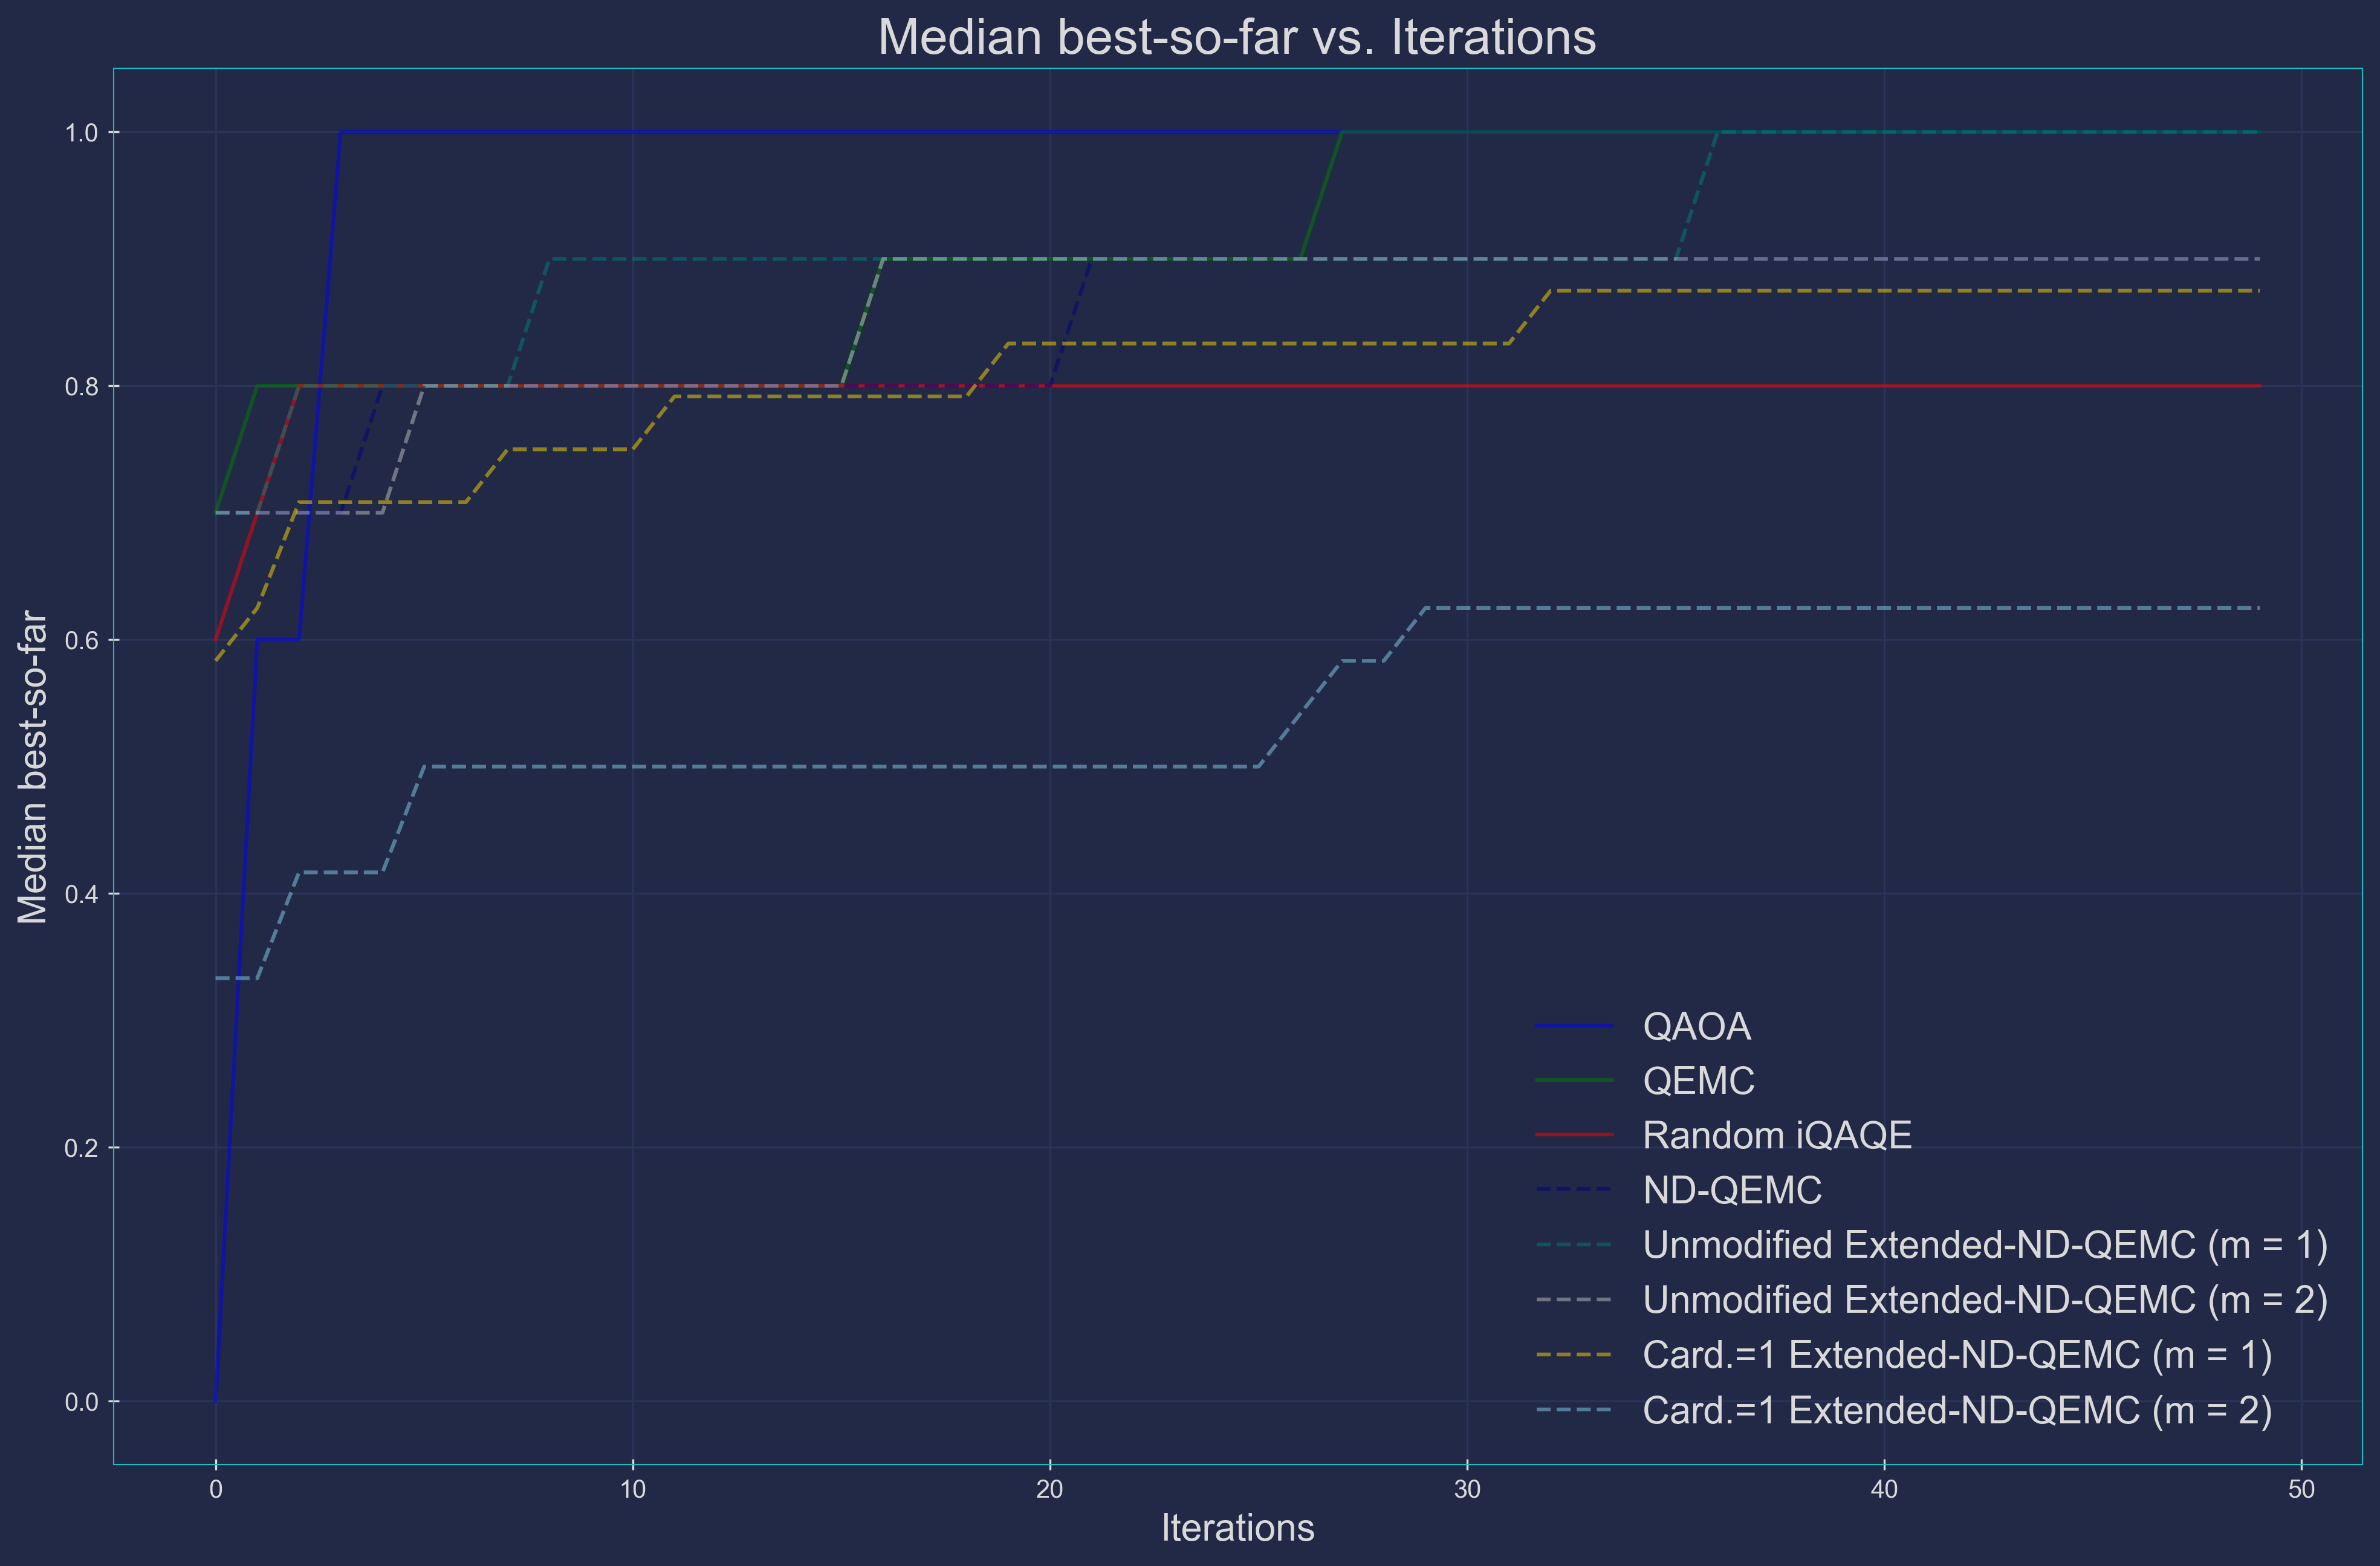
\includegraphics[width=1\textwidth, height=0.7\textwidth]{Figures/Appendix_A/8-node/Basic+ND_QEMC_Variations(8-node).png}
% 		\caption{Non-deterministic CNOT-gate-using schemes compared to \acrshort{qaoa}, \acrshort{qemc}, and a randomly chosen \acrshort{iqaqe} instance.}
% 		\label{fig:C_BSF_5_8-node}
% 	\end{subfigure}
%     \hfill
%     \begin{subfigure}[t]{0.495\textwidth}
% 		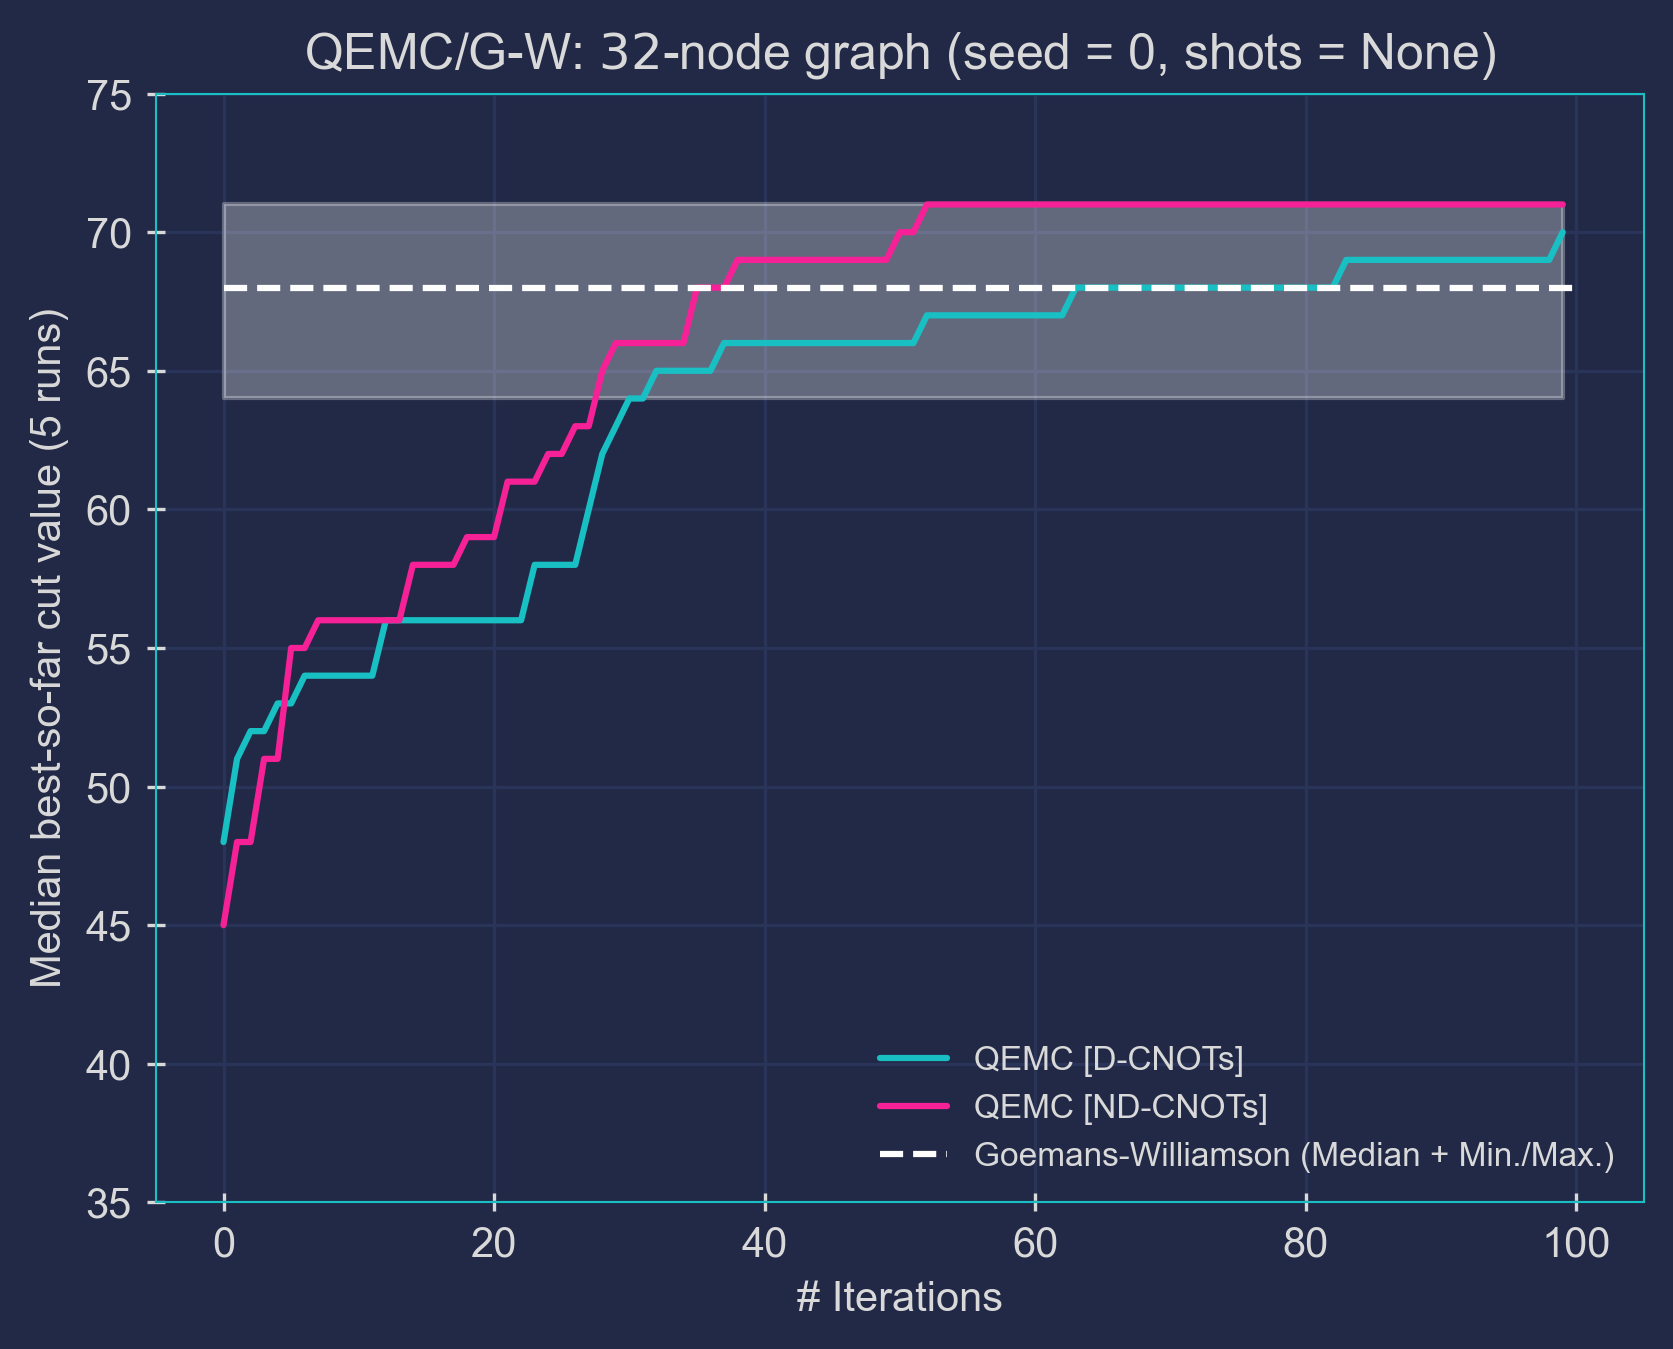
\includegraphics[width=1\textwidth, height=0.775\textwidth]{Figures/Appendix_A/32-node/32-node_Graph(QEMC&G-W)_Updated.png}
% 		\caption{$32$-node graph – \acrshort{qemc} and \acrshort{gw} exclusively.}
% 		\label{fig:C_BSF_1_32-node}
% 	\end{subfigure}

%     \bigskip

%     \begin{subfigure}[t]{0.495\textwidth}
% 		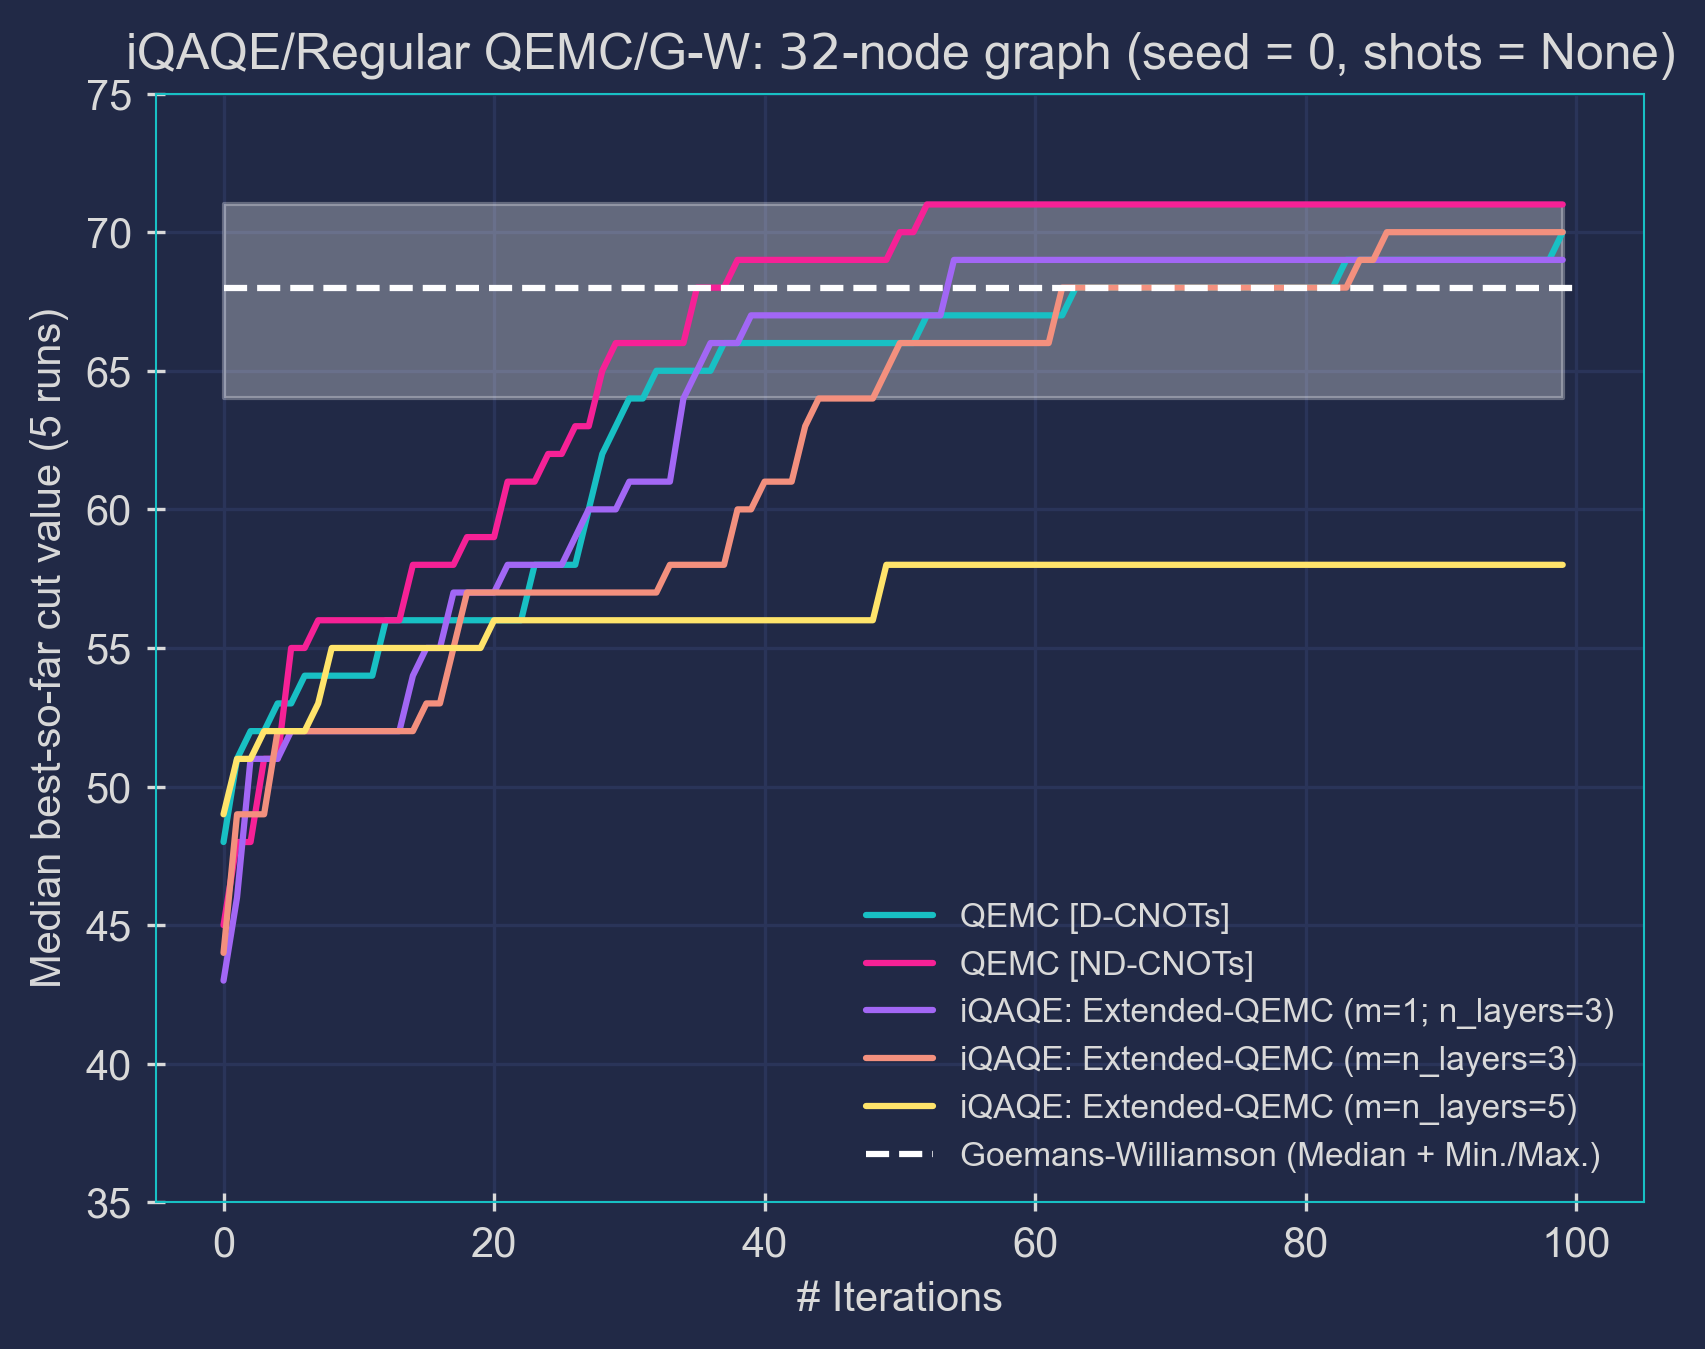
\includegraphics[width=1\textwidth, height=0.775\textwidth]{Figures/Appendix_A/32-node/32-node_Graph_Updated.png}
% 		\caption{$32$-node graph – other schemes.}
% 		\label{fig:C_BSF_2_32-node}
% 	\end{subfigure}
%     \hfill
%     \begin{subfigure}[t]{0.495\textwidth}
% 		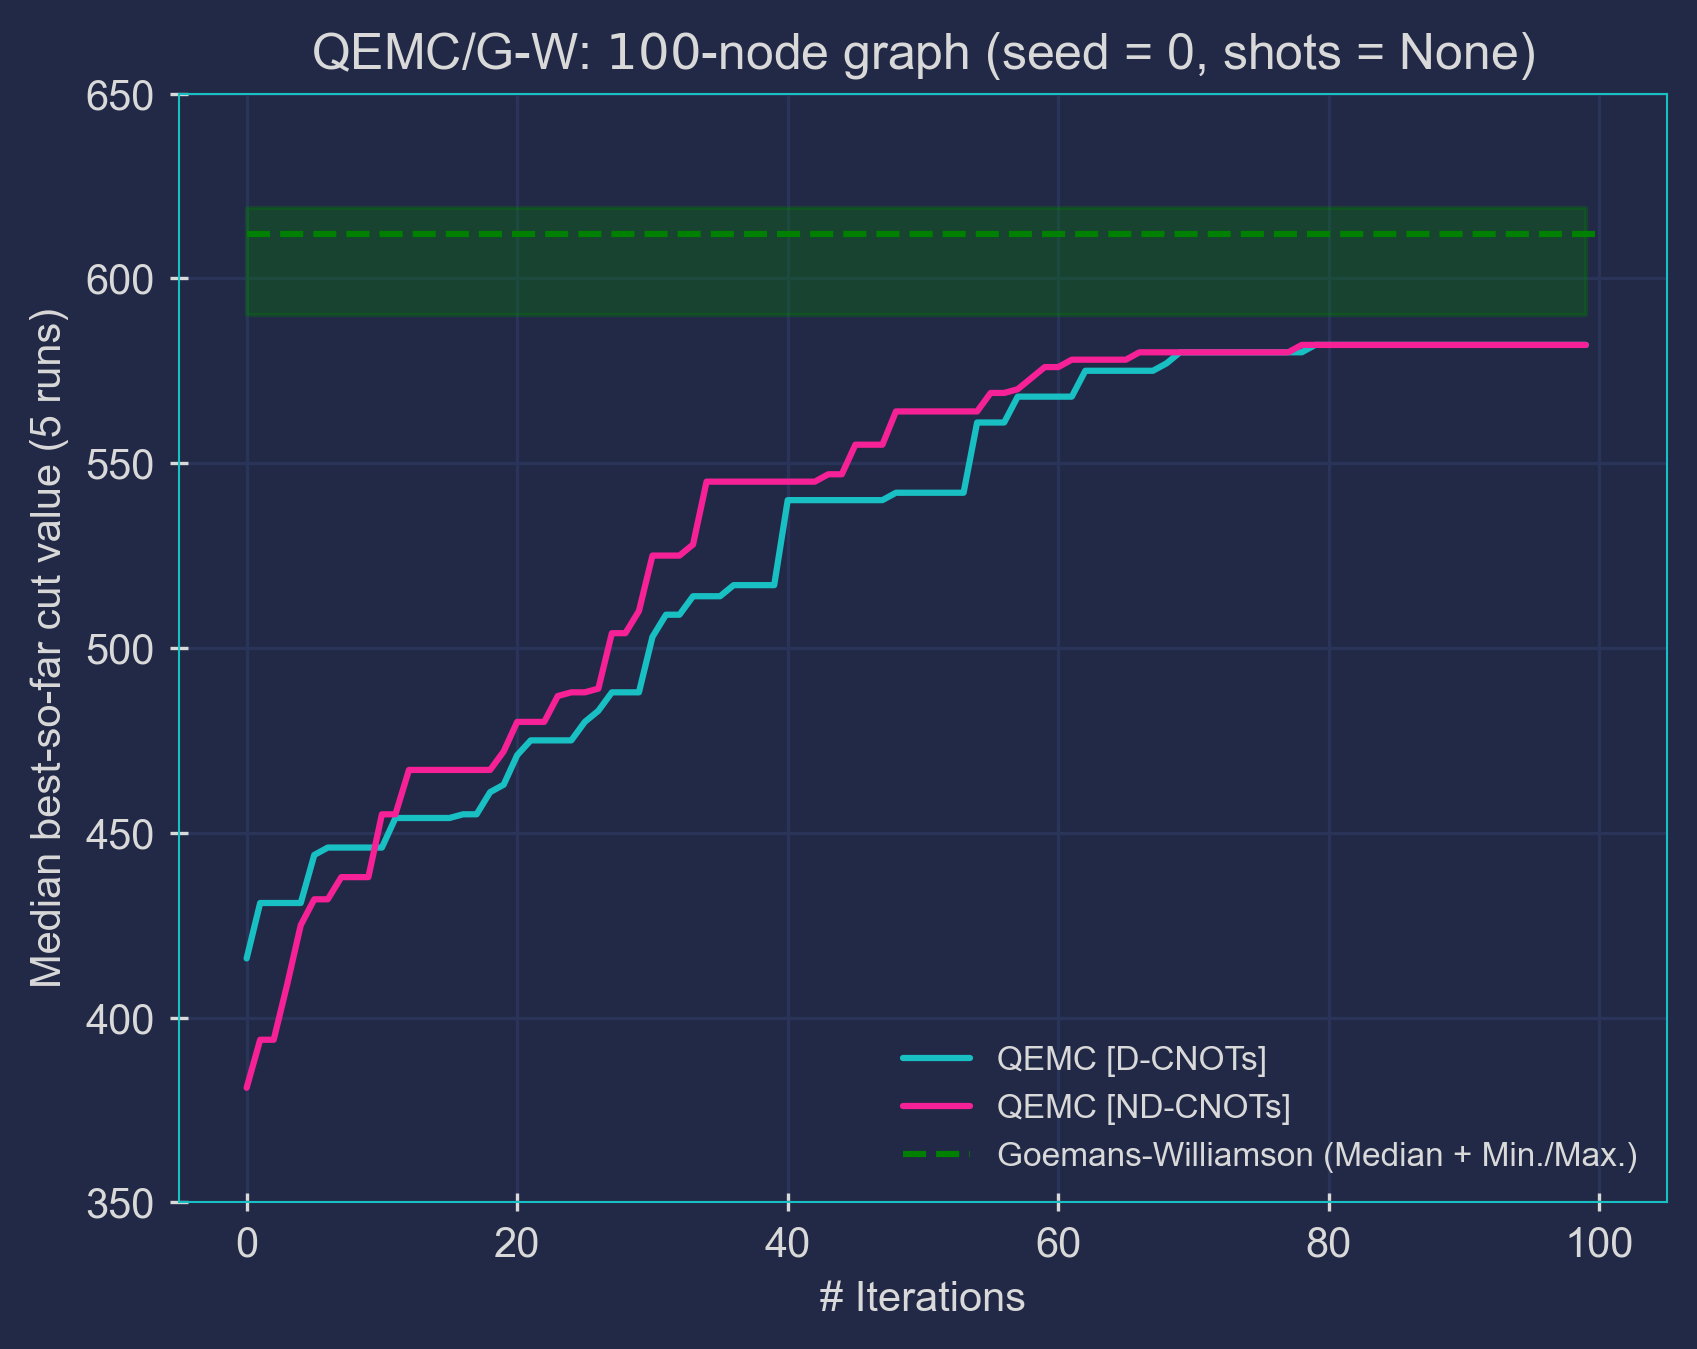
\includegraphics[width=1\textwidth, height=0.775\textwidth]{Figures/Appendix_A/100-node/100-node_Graph(QEMC&G-W)_Updated.png}
% 		\caption{$100$-node graph – \acrshort{qemc} and \acrshort{gw} exclusively.}
% 		\label{fig:C_BSF_1_100-node}
% 	\end{subfigure}

%     \bigskip

%     \centering
%     \begin{subfigure}[t]{0.495\textwidth}
% 		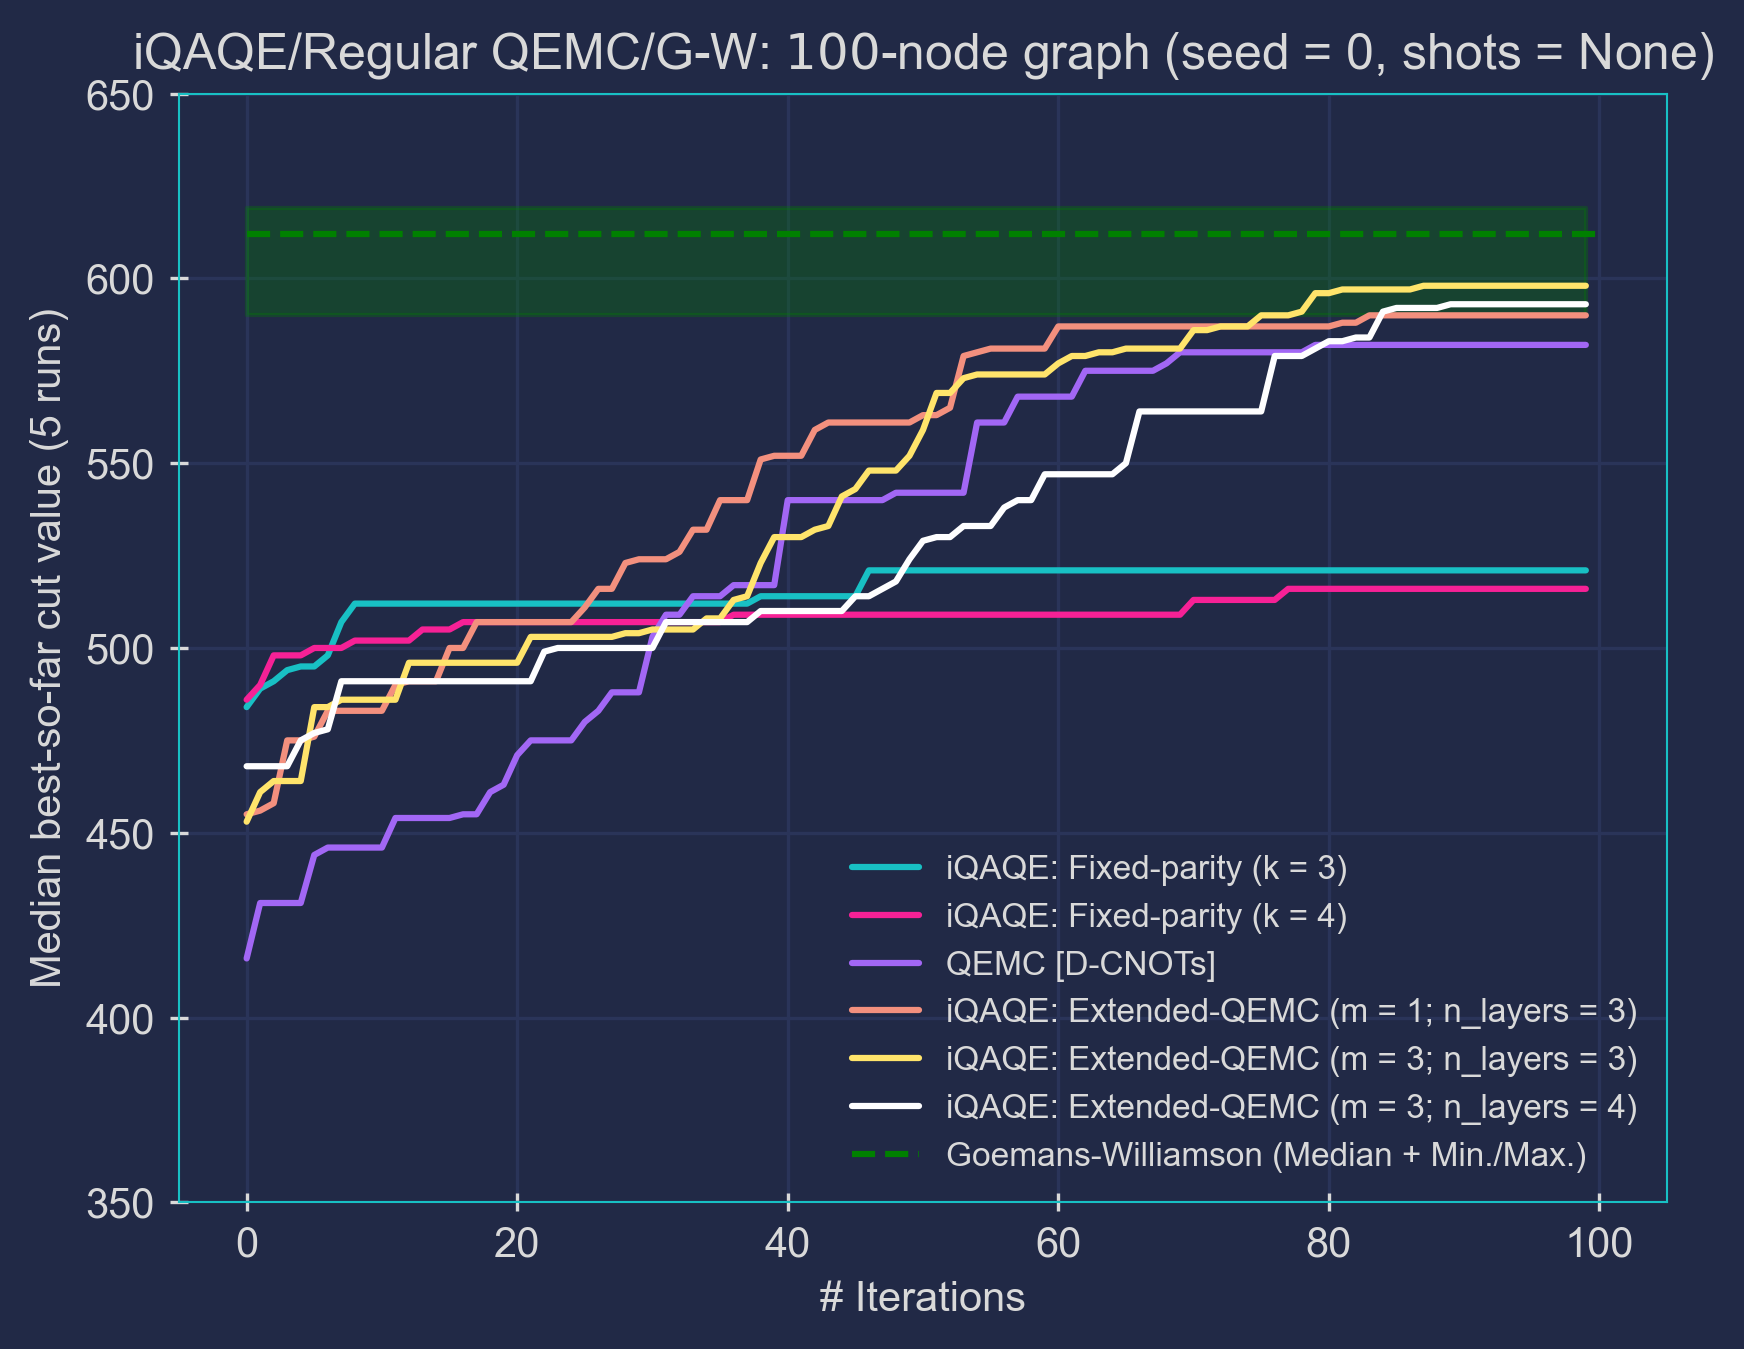
\includegraphics[width=1\textwidth, height=0.775\textwidth]{Figures/Appendix_A/100-node/100-node_Graph_Updated.png}
% 		\caption{$32$-node graph – other schemes.}
% 		\label{fig:C_BSF_2_100-node}
% 	\end{subfigure}

%     \caption{Revised results using the corrected median best-so-far metric for the $8$, $32$ and $100$-node graphs.}
%     \label{fig:Corrected_BSF_Results}
% \end{figure*}
